\documentclass[11pt]{article}

% MOTOR paper (SCORE #98). Same class, packages, margins and bibliography style as SCORE's paper (SCORE's paper/score/arxiv/main.tex).
% Build: tectonic -X compile --keep-intermediates main.tex (paper/CLAUDE.md), then delete main.aux, main.out, main.log.
% The story is the one agreed with the owner on 2026-11-08, #98 comment 6723992362: two ecosystems, physical AI and
% biomechanics; SOMA physical AI's standard body, MyoFullBody a candidate standard musculoskeletal model, MOTOR the
% solver between the two standards (owner, 2026-11-08). The main body has five sections (related work, method, results,
% discussion, conclusion; owner, 2026-11-18: results and conclusion fuller, the discussion beyond limits, the full
% formulas of the calibration and of the solver at inference time, better figures), and is at most 4 pages
% (it ends at \label{endofmain}) and follows the structure and register of the author's published paper (arXiv:2607.17639,
% cited as kardolus2026direct) for structure and tone only; none of its method is used here.
% Every number is read from a source named in a comment beside it. MOTOR is the per-frame solver (owner, 2026-11-09,
% recorded on #98: "report the fast per-frame solver as the result and make the whole-trial solve future work"); its
% results are the LabValidation run of 2026-11-07 with its residual reduction and physics run again on 2026-11-09 after
% fixes 18fed046 and 202bd660 (paper/motor/evidence/moments-labval-2026-11-09.txt, "after (all its trials)" columns,
% 716 of 720); measures that file does not hold (EMG per channel, vasti symmetry, signed offsets, time per step) are the
% 2026-11-07 run's (paper/motor/evidence/labval-final-2026-11-07.txt), said where they are used. Every comparison with
% OpenCap is measured as OpenCap measures it (same activities, activities weighted equally, its camera positions):
% paper/motor/evidence/comparison-2026-11-09.txt, the same 716 runs re-scored (#98 comment 6744969345). The whole-trial
% solve appears only as future work in the discussion, its numbers from paper/motor/evidence/motor-labval-2026-11-09.txt.
% OpenCap's numbers are its published ones; neither OpenCap nor PBL was rerun here.
\usepackage{iftex}
\ifPDFTeX
  \usepackage[T1]{fontenc}
  \usepackage[utf8]{inputenc}
  \usepackage{lmodern}
  \usepackage{textcomp}
\else
  \usepackage{fontspec}
\fi
\usepackage{amsmath,amssymb}
\usepackage{longtable,booktabs,array,calc}
\usepackage{graphicx}
\usepackage{xcolor}
\usepackage{tikz}
\usetikzlibrary{positioning,arrows.meta,fit,backgrounds}
\pgfdeclarelayer{back}\pgfsetlayers{back,background,main}
\usepackage[numbers,sort&compress]{natbib}
\usepackage{microtype}
\usepackage{placeins}
\usepackage{caption}
\captionsetup{font=footnotesize,skip=4pt}
\usepackage[margin=2cm]{geometry}
\usepackage[colorlinks=true,linkcolor=blue,citecolor=blue,urlcolor=blue]{hyperref}
\setlength{\emergencystretch}{3em}
\makeatletter\def\fps@figure{tp}\def\fps@table{tp}\makeatother
\renewcommand{\topfraction}{0.9}\renewcommand{\textfraction}{0.1}\renewcommand{\floatpagefraction}{0.8}
\setlength{\textfloatsep}{8pt plus 2pt minus 2pt}

\newcommand{\dg}{\ensuremath{^\circ}}
\makeatletter
\renewcommand\section{\@startsection{section}{1}{\z@}{-2.4ex \@plus -.6ex \@minus -.2ex}{1.4ex \@plus .2ex}{\normalfont\Large\bfseries}}
\renewcommand\paragraph{\@startsection{paragraph}{4}{\z@}{1.6ex \@plus .5ex \@minus .2ex}{-1em}{\normalfont\normalsize\bfseries}}
\makeatother
\AtBeginDocument{\setlength{\abovedisplayskip}{6pt plus 2pt minus 2pt}\setlength{\belowdisplayskip}{6pt plus 2pt minus 2pt}}


\title{\vspace{-1.5em}MOTOR: Musculoskeletal Optimisation Through Open Robotics Simulation}
\author{J.P. Kardolus, Babon Innovations B.V., Utrecht, The Netherlands}
\date{Working draft, 18 November 2026\vspace{-0.8em}}

\begin{document}
\maketitle

\begin{abstract}
\noindent Physical AI now estimates and generates moving human bodies at a scale that biomechanics has never had,
yet every bridge between the two fields is a custom chain, built for one body model and one route. We present MOTOR,
an open solver that takes the standard body of physical AI, SOMA, to the musculoskeletal model MyoFullBody and returns
its joint angles in the ISB convention, its joint moments, the ground reaction forces and the force in each of its 416
muscles, all solved on the GPU with Newton and MuJoCo Warp. From a single phone on OpenCap's LabValidation cohort,
MOTOR's joint angle error outside drop jumps is 5.6\dg{} (OpenCap Monocular: 4.8\dg) and its error in vertical ground
reaction force is 13.3\% of body weight (two-camera OpenCap: 11.4\%), at a median of 66\,s of solving per recording on
one GPU, against 44 to 70 minutes for OpenCap's recorded solves. Given laboratory inputs, its joint moments outside
drop jumps are within 0.4 to 0.8\% of body weight times height, so most of the remaining error comes from the
monocular input.
\end{abstract}
% Abstract numbers: paper/motor/evidence/comparison-2026-11-09.txt ("Cam1", mean, no drop jumps: angles15 5.62;
% "Cam1+Cam3": mean, 4 activities: vert 13.29; OpenCap's published figures, its last section: angles 4.8 (Monocular),
% vertical 11.4). 66 s: labval-final-2026-11-07.txt ("sim body wall seconds per step": total median 66.214 s);
% OpenCap's solves 2635 to 4196 s (44 to 70 min): our timing of the solves recorded in its LabValidation release, #98
% comment 6696117098. 0.4 to 0.8: moments-labval-2026-11-09.txt, section 1, "1 lab kin + lab grf" (walking 0.66, trunk
% sway 0.80, squats 0.42, sit-to-stand 0.47). 416 muscles: evidence/model-2026-11-06.txt.

\begin{figure}[h]
\centering
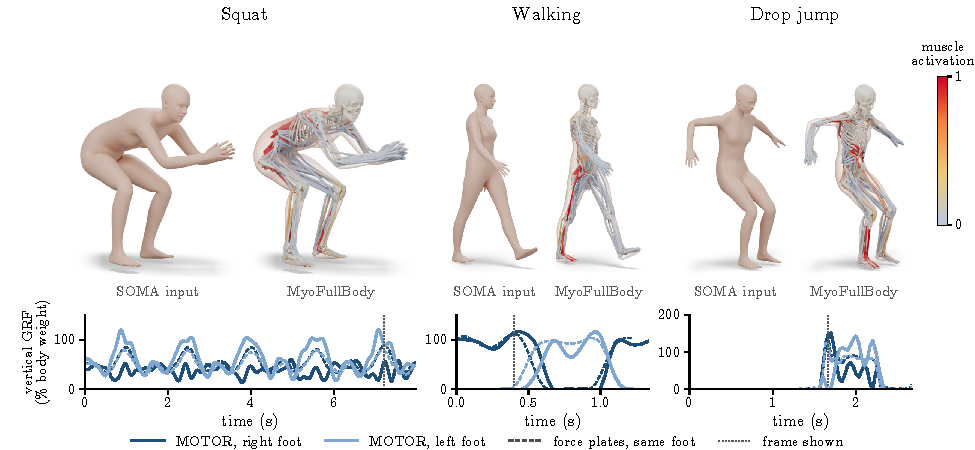
\includegraphics[width=0.55\linewidth]{figures/teaser.pdf}
\caption{MOTOR from the 45\dg{} camera: the SOMA body from GEM-X, MyoFullBody fitted inside its skin and coloured by
muscle activation, and each foot's vertical ground force (solid) against the force plates (dashed). The walk and the
drop jump were chosen as recordings whose force follows the plates most closely (1st of 27, 3rd of 52); the squat
(14th of 17) is shown at its deepest flexion. Median recordings are in Figure~\ref{fig:grf}.}
\label{fig:teaser}
\end{figure}
% Drawn from MOTOR's LabValidation run of 2026-11-07 (labval-final-2026-11-07.txt), trials subject2_squats1_Cam1
% (frame 216, the knee's deepest flexion, teaser-2026-11-07.json), subject3_walking2_Cam1 (frame 12, the right plate's
% peak) and subject4_DJ2_Cam1 (frame 50, the plates' summed peak); ranks among the 45 deg camera's trials by summed
% vertical MAE: walking2 1st of 27, DJ2 3rd of 52, the squat 14th of 17. Bodies: the demo clips' Blender passes
% (figures/demo render_clip.py); force series by the scorer's own path (tools.labval), filtered as OpenCap filters
% them, reproducing the run's report.json per-foot MAE and r. No participant video is shown (paper/CLAUDE.md).

\section{Related work}

Video-based estimators recover parametric bodies such as SMPL and MHR \cite{loper2015smpl,ferguson2025mhr} in world
coordinates from a single camera \cite{shin2024wham,shen2024gvhmr}, but their skeletons are not anatomical; SKEL
places an anatomical skeleton inside the skin of SMPL \cite{keller2023skel}. SOMA \cite{saito2026soma} unifies these
models by recovering one skeleton from SMPL, SMPL-X, MHR and others, and since GEM-X \cite{gemx} and Kimodo
\cite{rempe2026kimodo} now output SOMA bodies directly, SOMA has become the first standard body of physical AI.

Biomechanics estimates the forces of movement with software such as OpenSim \cite{delp2007opensim,seth2018opensim}.
OpenCap \cite{uhlrich2023opencap} fits an OpenSim model to keypoints from two or more phones and solves the kinetics by
tracking simulation in Moco \cite{dembia2020moco}, and OpenCap Monocular \cite{gilon2026monocular} works from a single
camera through WHAM and the learned force model GaitDynamics \cite{tan2026gaitdynamics}. The Portable Biomechanics
Laboratory (PBL) \cite{peiffer2025pbl} fits body scale and marker offsets over a whole session on MuJoCo's MJX, and B3D
\cite{cotton2026b3d} distils per-frame biomechanical fits of a MuJoCo model into a regressor on SAM-3D-Body; neither
estimates forces. Muscle forces are usually obtained by static optimisation \cite{crowninshield1981criterion}, which in
gait is practically equivalent to dynamic optimisation at a fraction of its cost \cite{anderson2001static}, or by direct
collocation \cite{degroote2016collocation}, and both run on the CPU. PhysPT \cite{zhang2024physpt} estimates ground
reaction forces from video, but on a rigid body without muscles.

On the GPU, MuJoCo Warp and Newton \cite{mujocowarp,newton}, both built on Warp \cite{warp}, simulate musculoskeletal
models such as MyoFullBody \cite{caggiano2022myosuite,li2026musclemimic} in parallel, and MuscleMimic and MS-Human-700
\cite{li2026musclemimic,wei2026mshuman} use them to train muscle-driven policies. These stacks learn to control a body;
none of them estimates the forces behind an observed movement. MOTOR applies them to that inverse problem
(Figure~\ref{fig:teaser}) and is, to our knowledge, the first open chain from video to muscle forces on Newton and
MuJoCo Warp.
% PBL, read 2026-11-08 at arxiv.org/html/2507.08268 ("Mujoco's GPU acceleration engine, MJX"; "jointly learning
% kinematics and body scaling and marker offset for the entire session"; "no inverse dynamics or kinetic estimation was
% performed"). B3D, read 2026-11-09 at arxiv.org/html/2608.29928 ("a stateless per-frame forward pass"). OpenCap
% Monocular: arXiv:2603.24733 (WHAM, GaitDynamics). B3D's head is supervised by Levenberg-Marquardt fits of a MuJoCo
% model to SAM-3D-Body's meshes (arXiv:2608.29928 abstract). PBL's licence: tools/labval/pbl/CLAUDE.md; owner, 2026-11-09.
% MyoFullBody's 416-muscle release: MuscleMimic (arXiv:2603.25544), cited with MyoSuite as myo_sim's README asks. New entries checked 2026-11-18 on their publishers' pages.
% Novelty claim and its scope: #98 comment 6683620930 ("Newton novelty").

\section{Method}
\label{sec:method}

MOTOR takes a body from physical AI and finds the musculoskeletal body that moved the same way, and then the forces
that moved it. Its input is a SOMA body for every frame of a recording: the posed skin $\mathcal{S}_t$, the rotation of
each body segment and the joint centres. Its model is MyoFullBody
\cite{caggiano2022myosuite,li2026musclemimic,holzbaur2005upper}, a whole-body model with 416 muscles whose bones are
sized to the person's SOMA segments. The model is fitted to the input in three ways at once: the rotation of each bone
group against its SOMA segment, anatomical landmarks on the bones against the same landmarks on the skin, and the bones
kept inside the skin. MOTOR has two parts that share this fit: a calibration, run once and offline, and a solver, run
on each recording (Figure~\ref{fig:method}, Appendix~\ref{app:method}).

How strongly each landmark should pull, and exactly where it sits on its bone, cannot be measured on a person. The
calibration therefore tunes these constants, which every body shares, on 21 synthetic SOMA bodies of varied build that
each perform seven clips, for which the right answer is known: bones that lie inside the skin and segments that turn
with the input. Writing $\Delta$ for the changes it tunes, each landmark's move on its bone and its weight's change,
both measured from the anatomical start, it solves
\begin{equation}
\Delta^\star=\arg\min_{\Delta}\;E_{\mathrm{skin}}(\Delta)+E_{\mathrm{rot}}(\Delta)+E_{\mathrm{start}}(\Delta),
\label{eq:calibration}
\end{equation}
\begin{equation*}
E_{\mathrm{skin}}=\sum_{c,r}\tilde D_{c,r}^{\,2},\qquad
E_{\mathrm{rot}}=\sum_{c,g}\tilde\Theta_{c,g}^{\,2},\qquad
E_{\mathrm{start}}=\sum_{i}\bigl(\Delta_i/\sigma_0\bigr)^2 ,
\end{equation*}
where $\tilde D_{c,r}$ is how deep the bones of region $r$ lie outside the skin in case $c$ and $\tilde\Theta_{c,g}$ the
rotation error of bone group $g$, each divided by its value at the start so that both count equally, and
$E_{\mathrm{start}}$ keeps each landmark's move $\Delta_i$ near zero ($\sigma_0=10$\,mm) within its bounds. No
measured joint angle enters it, and a result is kept only when bodies held out of the tuning score within 10\% of the
tuned ones.

At inference time, the solver first fits the person's own landmark moves from about 30 frames and then fits every
frame $t$, within the model's joint limits and couplings, as
\begin{equation}
q_t=\arg\min_{q}\;E_{\mathrm{rot}}(q)+\lambda_m E_{\mathrm{mark}}(q)+\lambda_s E_{\mathrm{skin}}(q),
\label{eq:fit}
\end{equation}
\begin{equation*}
E_{\mathrm{rot}}=\frac{1}{N_g}\sum_{g}\bigl\lVert\operatorname{Log}\bigl(R_g(q)^{\top}\hat R_{g,t}\bigr)\bigr\rVert^2,\qquad
E_{\mathrm{mark}}=\sum_{m}w_m\bigl\lVert p_m(q)-\hat x_{m,t}\bigr\rVert^2,\qquad
E_{\mathrm{skin}}=\frac{1}{N_b}\sum_{b}\bigl\lVert d_{b,t}(q)\bigr\rVert^2,
\end{equation*}
where $q$ are the model's joint coordinates, over $N_g$ bone groups and $N_b$ bone points; the same names as in Eq.~(\ref{eq:calibration}) mean the same errors, now for one frame.
$E_{\mathrm{rot}}$ matches the rotation $R_g$ of each bone group to that of its SOMA segment, $\hat R_{g,t}$;
$E_{\mathrm{mark}}$ pulls each landmark on the model, $p_m$, towards its point on the skin, $\hat x_{m,t}$, with its
calibrated weight $w_m$ (the weights summing to one); and $E_{\mathrm{skin}}$ pushes back in every bone point that lies
outside the skin by $d_{b,t}$. The calibrated $\lambda_m$ and $\lambda_s$ weigh the landmarks and the skin against the
rotations. All frames are
solved at once on the GPU with Newton and MuJoCo Warp \cite{newton,mujocowarp}, repeatably bit for bit.

The forces follow from the fitted motion. MuJoCo's inverse dynamics gives the torques each frame needs; the ground,
a plane fitted to the floor seen in the video \cite{wang2025moge2}, pushes only on skin points that touch it; and a
residual reduction in the manner of OpenSim's RRA \cite{delp2007opensim} adjusts the masses and the pelvis path
slightly, so that the ground can carry the movement. Static optimisation then divides the torques, as OpenSim does
\cite{crowninshield1981criterion}, in two stages: first the ground reaction forces from the balance of the pelvis
alone, then the activations of the 416 muscles at the least squared activation (Appendix~\ref{sec:forces}). What is
left unbalanced at the pelvis is recorded as the residual and judged against 2\% of body weight for force and 1\% of
weight times centre-of-mass height for moment, limits stricter than those Hicks et al.\ recommend
\cite{hicks2015model}.
% Eq. (fit): motor/fit/_frames.py weights (turns 1/N_g, markers MARKER_GOAL * trust / sum of trusts, MARKER_GOAL =
% 2.1169 written by level 1), segment ends' trust END_WEIGHT * mean landmark trust (motor/fit/__init__.py fitting(),
% END_WEIGHT = 2.1169), motor/fit/_skin.py (SKIN_GOAL = 1.0e3, winding number); couplings:
% motor/trial/_dynamics.py Coupled.applied, motor/fit/_card/_project.py COUPLING_TERMS = 5; GPU step:
% motor/fit/_card/_step.py, _solve.py; the same constants at the run's commit (SCORE 5996a8f2, inside/fit). Counts:
% evidence/model-2026-11-06.txt (416 muscles, 132 joints, 36 coupled). 84 landmarks: inside/landmarks/CLAUDE.md. Equal
% to mink (0.0025 deg, 0.0042 mm): #70 comment 6556935442.
% SCORE score/stages/sim_body/inside/tuning/__init__.py (constants :32-41, bounds :158-163, prior :166-170, weights
% :189-208, least_squares :313-314; GLOBALS marker goal and end weight); evaluation/__init__.py SKIN_ROWS = False;
% inside/tuning/CLAUDE.md ("Segment ends and two terms", owner 2026-11-03); 21 bodies x 7 clips (147 cases; tall,
% short, heavy, slim, long and short legs), clips and the held-out rule: #70 comment 6556935195; hybrid Jacobian (end
% columns by finite differences): #70 comment 6556935442 section 5, tuning/_differences.py hybrid.
% Level 2: motor/fit/_constants.py (residuals :106-126, bounds MARK_MOST = 0.03 :89-100), motor/fit/__init__.py
% SAMPLE = 30, motor/fit/_card/_level2_lm.py. Path: motor/model/__init__.py filtered; CUTOFF = 6.0:
% motor/solvers/__init__.py. Inverse dynamics: muscles/__init__.py needed (mj_rne + armature - passive).
% Contact as run (SCORE 5996a8f2, inside/contact/__init__.py): GAP = 0.005, STANCE_HIGH = 0.05, FRICTION = 0.5,
% closeness; the seen stance: tools/labval/CLAUDE.md (_soma.seen_stance); floor: commits 58c54d6f, 292d6f88. RRA
% (18fed046, as in motor/rra/__init__.py): RRA_ROUNDS 3, TRACK 0.01, MASS_MOST 0.02; rra/_cap.py; _gates.py FOLLOWED
% 5 deg, MOVE_MOST 0.02 m; limits RESIDUAL_FORCE, RESIDUAL_MOMENT. Static optimisation as run (SCORE 5996a8f2
% inside/muscles/__init__.py): BALANCE 100, CONTACT_COST 1e-3, SHARE_COST 0.03, SHARE_ROUNDS 2, staged(), problem()
% (moment arms zeroed on the root, mju_muscleGain/Bias, LIGAMENTS), nudge 1.0 at once against 5e-3 in two stages
% (the SHARE_COST comment, lines 28-34, #70 2026-11-05); SLIDE_MOST = 1.2 m/s and the sliding edge (contact :305,
% :329-332); limits RESIDUAL_FORCE, RESIDUAL_MOMENT and h_com: _gates.py; Hicks et al. 2015 (5 % and 1 % of the peak
% net external force);
% projected Newton: motor/solvers/__init__.py least. Bit for bit: commit e0c46164, evidence/speed-2026-11-06.txt.

\section{Results}
\label{sec:protocol}

OpenCap's LabValidation cohort \cite{uhlrich2023opencap} records healthy adults walking, squatting, rising from a
chair and drop-jumping, captured by five phones together with motion capture, force plates and EMG. GEM-X
\cite{gemx,li2025genmo} turned each of its 720 single-camera recordings of nine subjects into SOMA bodies, and MOTOR
solved every recording independently; 716 runs completed. Subjects 7 to 11 were held out and were never used to choose
a setting. Following OpenCap, errors are averaged over the four activities with equal weight and taken from its
cameras at $\pm45\dg$ (Appendix~\ref{app:protocol}); OpenCap's figures cover ten subjects, ours nine.
% Cohort: #98 comment 6683683998 (144 trials x five cameras = 720); 716 of 720: moments-labval-2026-11-09.txt
% (section 3); held out: labval-final-2026-11-07.txt (header); tuning on subjects 2-5: same file ("tuning", commit
% a40b66d6). The results are the run of 2026-11-07 with its residual reduction and forces solved again on 2026-11-09
% after fixes 18fed046 and 202bd660 (moments-labval-2026-11-09.txt, "after" columns), compared as OpenCap measures in
% comparison-2026-11-09.txt (#98 comment 6744969345); OpenCap's ten subjects: comparison-2026-11-09.txt ("Uhlrich et
% al. 2023 (two cameras, Table 1; 10 subjects)").


\begin{figure}[t]
\centering
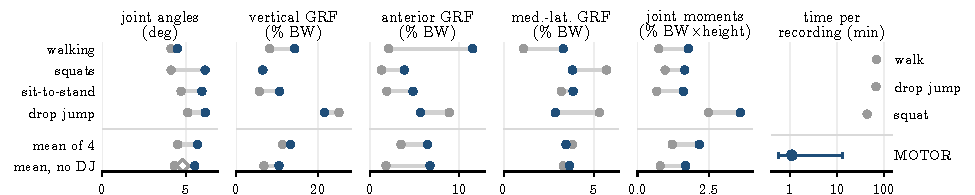
\includegraphics[width=\linewidth]{figures/summary.pdf}
\caption{Mean absolute error against the laboratory per activity, and solve time per recording. MOTOR pools its runs
from the two $\pm45\dg$ cameras and scores 15 angles (OpenCap 18); OpenCap Monocular reports angles only, without drop
jumps. Ground reaction force (GRF) is both feet summed. MOTOR's time is on one L4 GPU without pose estimation;
OpenCap's are its recorded solves.}
\label{fig:summary}
\end{figure}
% drawn by figures/summary/plot.py. data: comparison-2026-11-09.txt "Cam1+Cam3" (angles 4.48/6.13/5.94/6.14/5.67/5.52; vertical 14.32/6.55/10.63/21.65/
% 13.29/10.50; anterior 11.54/3.86/4.84/5.69/6.48/6.75; medio-lateral 3.30/3.81/3.85/2.86/3.45/3.65; moments
% 1.79/1.66/1.61/3.61/2.17/1.69) and its last section (Uhlrich et al. 2023 Table 1; Monocular 4.8); time:
% labval-final-2026-11-07.txt (66.214 s, 34.843 to 788.668) and #98 comment 6696117098 (4196, 4096, 2635 s).

From the 45\dg{} camera and outside drop jumps, MOTOR's joint angles are off by 5.6\dg{} on average over the fifteen
angles it shares with OpenCap Monocular, which reports 4.8\dg{} (Figure~\ref{fig:summary}). Most of that error is a
constant offset in each trial: once it is removed, the error falls to 3.1\dg, and the knee follows the laboratory with a
correlation of 0.98. The vertical ground reaction force of both feet together is off by 13.3\% of body weight, against
11.4\% for two-camera OpenCap; MOTOR does better in drop jumps (21.7 against 25.2\%) and worse in the other activities
(10.5 against 6.8\%). Each foot's force follows its plate in time (Appendix Figure~\ref{fig:grf}), though in this run
not its share of the load when both feet are down.
% comparison-2026-11-09.txt ("Cam1", mean no DJ, angles15 5.62; "Cam1+Cam3" mean no DJ 5.52; OpenCap's over "the
% same 18 DOF"; "Cam1+Cam3": mean 4 13.29 / 6.48 / 3.45; no DJ 10.50;
% drop jump vertical 21.65; OpenCap 4.3, 11.4 / 3.5 / 3.8, 6.8, drop jump 25.2; Monocular 4.8);
% moments-labval-2026-11-09.txt (after: "envelope" 5.16 [4.77, 5.59], cMAE 3.06; "held out 7-11, all" r 0.77 / 0.79);
% tab:angles (knee r 0.98-0.99).

The joint moments are off by 2.17\% of body weight times height, against OpenCap's 1.22\%. To see where that error
comes from, we swapped MOTOR's inputs for the laboratory's on 159 trials (Appendix Table~\ref{tab:moments-inputs}):
given the laboratory's motion and force plates, MOTOR's moments outside drop jumps are within 0.42 to 0.80\%, no worse
than OpenCap's from video, so most of the error comes from the monocular input rather than the solver. The pelvis
residual still exceeds its limits (median 7.2\% of body weight), the activations agree only weakly with EMG (mean $r$ of
0.23), and a recording takes a median of 66\,s of solving on one L4 GPU, against 44 to 70 minutes for OpenCap's recorded
solves.
% comparison-2026-11-09.txt (moments Cam1+Cam3 2.17, 1.69; OpenCap 1.22, 0.80); moments-labval-2026-11-09.txt section 1
% (159 trials: 1.28; 1.74; 2.24; 2.41) and "residuals (after)" (all: F 7.2, M 8.92, frames within 0.204);
% labval-final-2026-11-07.txt ("EMG per channel": vasti 0.36-0.42, mean r 0.23 also after the rerun; "sim body wall
% seconds per step": total 66.214 [34.843, 788.668], fit 21.825, residual reduction iterations 19.862); OpenCap's
% solves: #98 comment 6696117098.

\section{Discussion}

A single GPU solver thus carries a standard body from one phone to muscle forces on a public cohort, forty to sixty
times faster than OpenCap's recorded solves.
% 4196 / 66.2 = 63 (walk), 2635 / 66.2 = 40 (squat); moments-labval-2026-11-09.txt section 1 ("each leaves about half";
% lab inputs walking 0.66, trunk sway 0.80, squats 0.42, sit-to-stand 0.47).
In this run its largest remaining error was the division of the load between the feet. In squats the division alone
accounts for an error of 16.2\% of body weight (the per-foot error is 16.4\% and the error of the total force 3.2\%),
and the summed force follows the plates ($r=0.98$) while each foot does not (0.41 and 0.39). The balance of the pelvis
fixes the total force but not how it is divided, and the division followed the lean of the input body: its error
changes sign with the camera, from $+0.07$ to $-0.07$ in the left foot's share, although the model itself is symmetric.
The input also carries the anterior error, since the anterior force that the video's motion demands is 17.4\%
of body weight off the plates against 2.6\% for the laboratory's, and the elbows come out 21 to 24\dg{} too straight,
as they are in GEM-X's output.
% motor issue #1 comment 6931271320 (715 runs of 11-07: squats per-foot 16.4, split part 16.2, total part 3.2, MAEs of
% two components, not additive; summed r 0.98, per foot
% 0.41 / 0.39); #1 comment 6975016712 (left share per camera, squats +.07 ... -.07; model 20.71 against 20.69 kg per
% side); moments-labval-2026-11-09.txt section 2 (17.4 against 2.6); labval-final-2026-11-07.txt ("signed offsets":
% elbow -21.12 / -23.66); elbow-2026-11-07.txt (median -18.5); comparison-2026-11-09.txt (KAM Cam1 1.97, Monocular
% 0.36); #98 comment 6721835197 (37-44 against 9-16 mm); teaser-2026-11-07.json (90.13 left / 52.93 right).

Two changes made since this run address the division; both have so far been measured on subsets and still await a run
on the full cohort. The first takes each foot's contact from its lowest skin point above a floor fitted per trial,
instead of from GEM-X's stance flag, and lowers the per-foot vertical error of 18 held-out walks from 17.2 to 15.1\% of
body weight. The second adds a row to the static optimisation that hands the load from one
foot to the other across double support. With it each foot's force follows its plate: on 14 trials of subjects 2 to 4
the per-foot root-mean-square error falls from 16.1 to 13.2\% of body weight in walking and from 13.5 to 6.1\% in
squats, although the pelvis residual moment rises by 7 to 11\,N\,m. A whole-trial solve raised the share of frames within the residual limits
from 21 to 35\% at five times the cost but worsened the moments and the agreement with EMG, so the next gains lie in
the input. Three limitations remain: the
cohort contains only healthy adults, GEM-X resamples every clip to 30\,Hz although drop jumps carry the largest errors,
and the calibration in use has no recorded held-out score.
% ad7e8c6: motor issue #1 comment 6962132074 (held-out Cam1 walking n = 18: 17.2 -> 15.1). 6d72d73: #1 comment
% 6980387981 (13 trials, subjects 2-4, Cam1: squats per-foot RMSE 21.2 -> 13.5). Hand-over split 4799331: #1 comment 6985456815 (14 trials, subjects 2-4, Cam1, 175ab04 -> 4799331: RMSE walking 16.1 -> 13.2, squats 13.5 -> 6.1, sit-to-stand 17.4 -> 11.3, drop jump 30.5 -> 26.6; left-share MAE walking 0.184 -> 0.062; residual moment +7 to +11 N m; dip and landing peaks from the input's CoM acceleration). Neither is in the full-cohort
% results above; drop jumps 19.9 -> 19.8 (#1 comment 6962132074); 6d72d73 against ad7e8c6, SPLIT swept on the same 13
% trials, pelvis residual moment +1.5 to +6 N m (#1 comment 6980387981). Whole-trial solve:
% evidence/motor-labval-2026-11-09.txt (frames within, all trials 0.349 against 0.206, envelope 0.396 against 0.203;
% envelope moments 2.03 [1.93, 2.12] against 1.77 [1.68, 1.86], EMG r 0.16 against 0.23; 308.563 against 66.214 s). B3D Table 2 (3.66 against 3.24 deg). Drop jumps:
% moments-labval-2026-11-09.txt (after, 3.51). Calibration: #70 comments 6621931172, 6629418159 (5.15 %), 6565739270.
% 30 Hz: tools/labval/_soma.py RATE.

\enlargethispage{3\baselineskip}
\section{Conclusion}

From one phone, MOTOR estimates joint angles within 5.6\dg{} and the summed vertical ground reaction force within
13.3\% of body weight, in about a minute per recording. Markerless methods moved the estimation of movement's forces
out of the laboratory; MOTOR moves it out of the bespoke chain, so that every better body from physical AI carries
into forces that biomechanics can study at scale.
% Every float of the main body is placed before this point.
\FloatBarrier
\label{endofmain}

\bibliographystyle{unsrtnat}
\bibliography{references}

\clearpage
\appendix
\section{The method in full}
\label{app:method}
\begin{figure}[h]
\centering
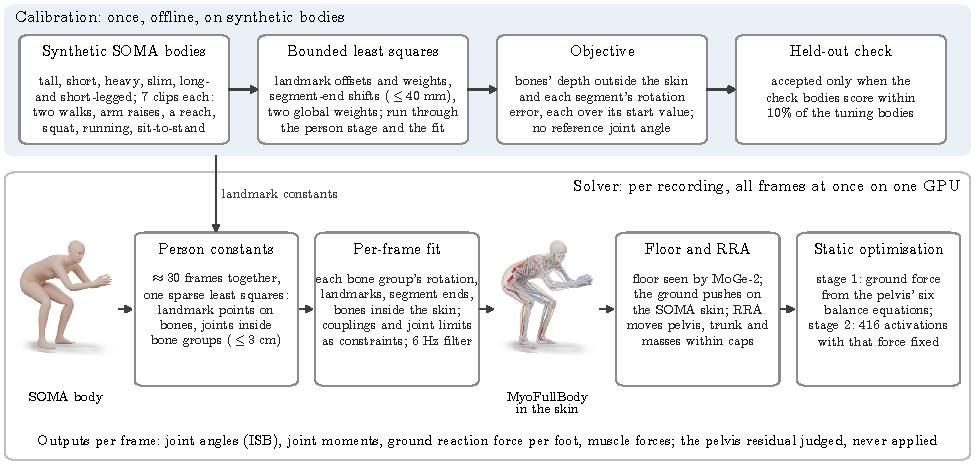
\includegraphics[width=\linewidth]{figures/method.pdf}
\caption{MOTOR's two layers: the calibration (Eq.~\ref{eq:calibration}) once on synthetic bodies, and per recording
the person's constants (Eq.~\ref{eq:person}), the fit (Eq.~\ref{eq:fit}), the residual reduction (Eq.~\ref{eq:rra})
and static optimisation (Eqs.~\ref{eq:so}, \ref{eq:stages}), each over all frames at once on one GPU.}
\label{fig:method}
\end{figure}
% Drawn for this draft from the Method section and Appendix A; thumbnails: the squat's frame 216 skin and inside passes
% (subject2_squats1_Cam1, the 2026-11-07 run).

This appendix sets out the method in the order in which it runs (Figure~\ref{fig:method}, Section~\ref{sec:method}). The input body and the
model are described first, then the correspondence between them and the fit that both later stages share. The
calibration, done once and offline, follows, and finally the solver that runs on every recording: the person's
constants, the per-frame fit, and the forces solved on the fitted path. Figure~\ref{fig:skin} shows
the fitted model inside the skin, at full size, in two poses.

\begin{figure}[p]
\centering
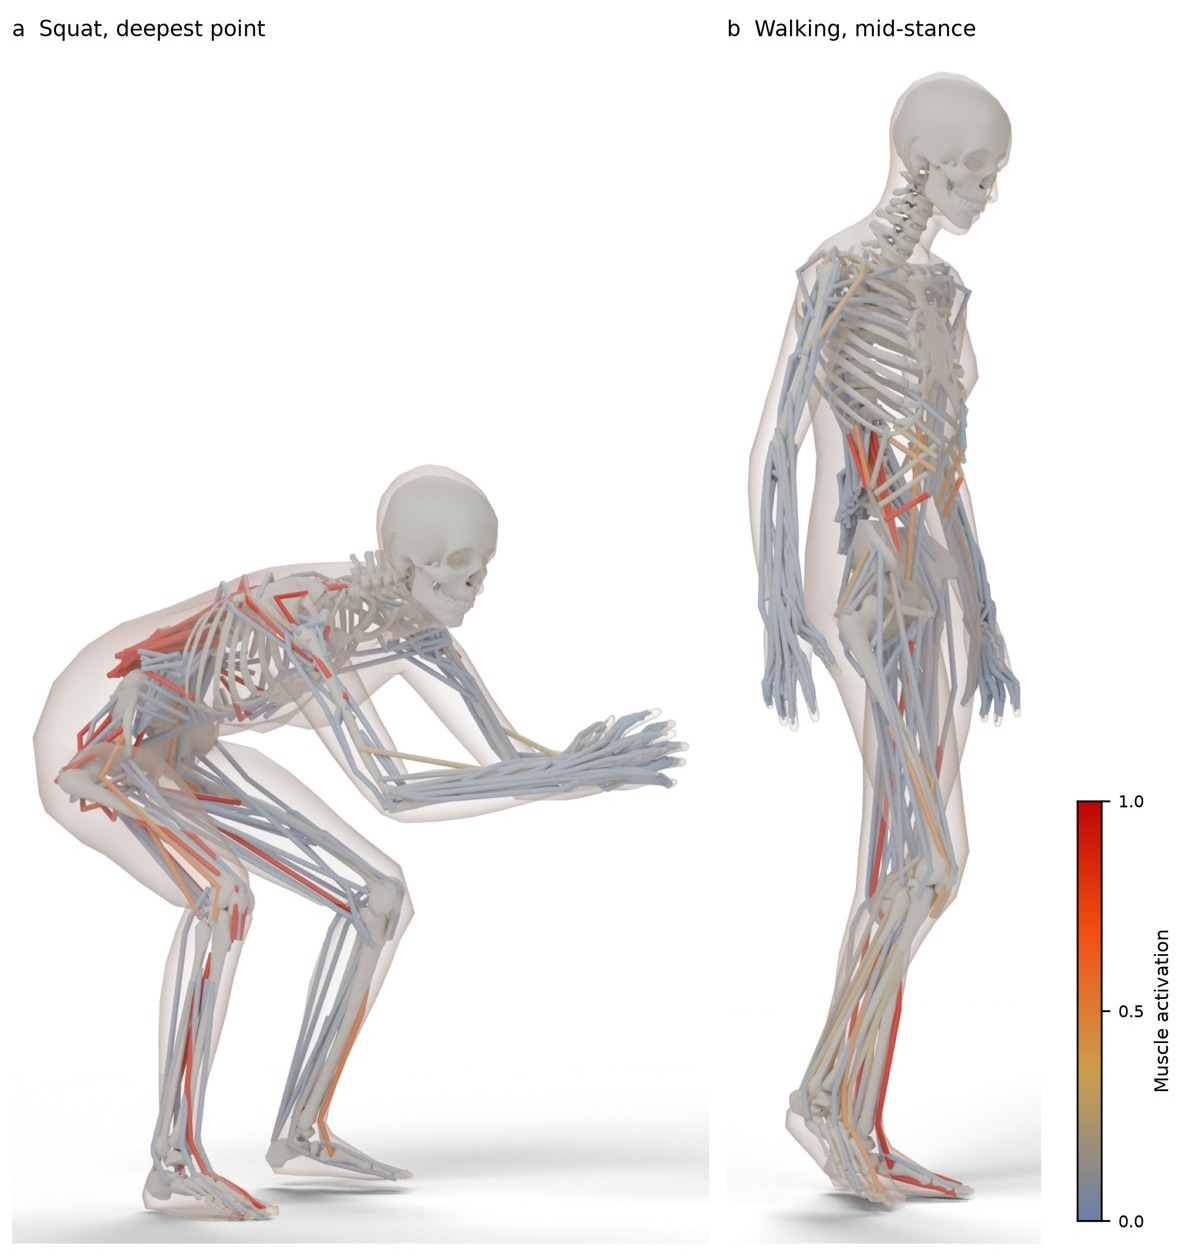
\includegraphics[width=\linewidth]{figures/simbody-in-skin.jpg}
\caption{MyoFullBody fitted inside a person's skin from one LabValidation video: (a) a squat at its deepest point,
(b) walking at mid-stance. Drawn from MOTOR's saved LabValidation results, the muscles coloured by MOTOR's
activations.}
\label{fig:skin}
\end{figure}
% Figure added in commit 244bae78 from MOTOR's saved LabValidation results; its trials are not recorded there.
% Cropped of its empty top band for this draft.

\subsection{The input body}

Any source that provides a skin mesh, segment rotations and joint centres can supply MOTOR's input, although only
SOMA bodies, from GEM-X and Kimodo, have so far been run. In the validation the source is GEM-X
\cite{gemx,li2025genmo} applied to one smartphone video. GEM-X gives a SOMA body \cite{saito2026soma} per frame,
consisting of its identity (shape), root translation and global segment rotations, at 30\,Hz, the rate to which
GEM-X resamples every clip. MOTOR takes this body as given and never changes its shape or pose. GEM-X is given the
camera's field of view, which MoGe-2 \cite{wang2025moge2} estimates from the same video, and its own contact
post-process holds the standing feet still. Because GEM-X's output has no floor, the floor is estimated from the
video: a plane is fitted to MoGe-2's points of the floor beside the person, the whole clip is rotated rigidly so that
this plane is level, and the clip is lowered until the lowest point of its feet touches it.
% tools/labval/_soma.py (RATE = 30.0, "its motion-video normalises every clip to 30 Hz") and tools/labval/CLAUDE.md
% (commit d6ac3b5d); field of view and seen floor: tools/labval/CLAUDE.md ("The floor is seen, not assumed"),
% commits 58c54d6f and 292d6f88 (#98).
% Kimodo bodies run: score/stages/sim_body/CLAUDE.md (the sim body stage solves each scene's clips).

\subsection{The musculoskeletal model}

The model is MyoFullBody from MyoSuite \cite{caggiano2022myosuite}, its arm and hand taken from MoBL-ARMS
\cite{holzbaur2005upper,saul2015benchmarking}. It has 416 muscles, 86 bones and 132 joints, of which one is the free
root, 36 are coupled to another joint by a polynomial (those of the knee and the shoulder girdle, for example) and 95
move freely. Its bone groups (below) are sized to the person's SOMA body, each group's length taken from its SOMA
segment, joint to joint, so that MOTOR solves for no length. Its masses are SOMA's segment volumes distributed over the
subject's measured mass.
% Counts: paper/motor/evidence/model-2026-11-06.txt (MuJoCo 3.15.0 on the sized model file). Sizing and masses:
% score/stages/sim_body/inside/fit/CLAUDE.md ("No size unknowns": lengths from inside/sizing), inside/volumes.

\subsection{Segments, bone groups and landmarks}

\paragraph{Segment rotations and bone groups.} Each SOMA segment is coupled to a \emph{bone group}, the bones of
MyoFullBody that cover the same part of the body, one of which, the group's \emph{frame bone}, carries the segment's
rotation (Appendix~\ref{app:parameters}). A spine segment is coupled to the vertebrae at its height, paired by their
share of the spine's height, and the hand to the bones of the wrist and hand, with the lunate carrying its rotation.
Each segment drives one group. SOMA has two neck segments where MyoFullBody has a single rigid neck; the first drives
it, and the second drives nothing, although its rotation error is still reported.

How a segment's frame lines up with its group's frame is read once from the two models at rest (SOMA's template in its
bind pose, MyoFullBody in its default pose with its couplings applied) and kept as a fixed \emph{rest alignment} per
group. Each group's anatomical axes are constructed on both models from the same anatomy: the line between the
group's end joints or between landmarks, the bone's own axis, or a hinge line, such as the line through the first and
fifth metatarsal heads that the foot and toes share. The feet are then turned about that hinge line until SOMA's foot,
flat on its floor at rest, corresponds to MyoFullBody's heel bone flat in its default pose, and the groups whose bones
would stand outside SOMA's skin along those lines (the head first) are turned and shifted rigidly at rest to their
least depth outside it. The rest alignment is therefore geometry of the two models: it is never fitted to motion data
or to any reference joint angle, and never per person or per clip.
% score/stages/sim_body/inside/bone_groups (GROUPS) and inside/calibration (its CLAUDE.md: read at rest by aligning
% anatomical axes, REFERENCES, HINGED, LONG_LINES, LEVELLED, INSIDE_GROUPS; "Never fit it, never per person or per
% clip"); one to one: inside/fit/CLAUDE.md ("One segment drives one bone group", owner 2026-11-01); hand under the
% lunate: fit/__init__.py HAND_TOP.

\paragraph{Virtual markers on anatomical landmarks.} Beside the rotations, the fit uses virtual markers on anatomical
landmarks, each defined by its anatomy following the ISB recommendations \cite{wu2002isb,wu2005isb}: the acromion, the
humeral epicondyles, the anterior and posterior superior iliac spines, the malleoli, the metatarsal heads and others.
Each landmark sits on a fixed point of the SOMA mesh, given as a face and barycentric weights, so that it moves with
the person's skin, and on the matching point of a MyoFullBody bone, plus an offset from the bone toward the skin. A
study of the two models placed 102 landmarks, of which the fit uses 84, each with its own weight. No licensed
dataset's marker list is used.
% score/stages/sim_body/inside/landmarks/CLAUDE.md (102 from the landmark study of 2026-10-29, 84 the solver's; every
% point by its anatomical definition, never a licensed dataset's marker list).

\paragraph{Joint centres as segment ends.} SOMA's rig joints mark where each bone group begins and ends: the hips,
knees, ankles, shoulders, elbows, wrists and the joints between spine segments. Each such end acts as one more marker,
placed at MyoFullBody's own joint centre there and aimed at SOMA's joint. The joints inside a group (the lumbar
levels, the shoulder blade, the wrist bones and the joints of the inner foot) are aimed at nothing; the landmarks and
the model's couplings place them. No joint is treated as a special case.
% inside/fit/CLAUDE.md ("SOMA's group ends are a target", #70, the owner's plan 2026-10-29).

\paragraph{The skin.} The bones belong inside the body from which they came. SKEL builds this idea into a body model,
a biomechanical skeleton placed inside the skin of SMPL \cite{keller2023skel}; MOTOR instead uses the input's own skin
as a target. Each frame's SOMA skin is posed, and a fixed subset of the vertices of every bone mesh is measured against
it: each vertex's offset to the closest point of the skin, or zero when the vertex lies inside, as decided by the
generalised winding number \cite{jacobson2013winding}.
% inside/fit/CLAUDE.md ("Level 3 holds the bones inside the skin; level 2 does not", owner 2026-11-01); fit/_skin.py.

\subsection{The fit}
\label{sec:fit}

Fitting the solver, Equation~\eqref{eq:fit}, is the objective that the calibration and the solver on every recording
share. For one frame, with the person's constants fixed, it finds MyoFullBody's coordinates $q$
that come closest to the input body while every joint stays within its anatomical limits.
The first term is the main one: for each of the $N_g$ bone groups, it measures the angle between the frame bone's
orientation $R_g(q)$ and its SOMA segment's rotation $\hat R_g$ composed with the group's rest alignment. The second
pulls each marker $m$ (the landmarks and the segment ends) at its point $p_m(q)$ on the model toward its point $\hat
x_m$ on the SOMA body, weighted by $\bar w_m$, its weight $w_m$ over the sum of all. The third holds the $N_b$ bone
vertices inside the skin, $d_b$ being a vertex's offset outside it. Each goal is normalised by its own count, as OpenSim's inverse kinematics weighs its goals
\cite{seth2018opensim}. The markers' goal $\lambda_m$ is set by the calibration (2.1169), and the skin goal
$\lambda_s$ is $10^3$, chosen in a sweep that traded the bones outside the skin against the rotation error. A coupled
joint (a \emph{follower}) moves with a \emph{leading} coordinate through MyoFullBody's own polynomial $f$, held as an
equality constraint, and the limits are the published ranges of the leading coordinates, held as bounds. The fingers
are held at SOMA's rest.
% Form and weights: inside/fit/CLAUDE.md ("Weights are OpenSim's IK's", "Reuse, not handwritten maths"); MARKER_GOAL =
% 2.1169: score/stages/sim_body/inside/fit/_frames.py; SKIN_GOAL = 1.0e3: inside/fit/_skin.py and the sweep in
% inside/fit/CLAUDE.md ("The skin goal, swept"); #70 comment 6556935195 (method record, part 1); fingers at SOMA's
% rest: #70 issue body (status) and inside/fit/CLAUDE.md (DofFreezingTask for the fingers).

The reference solver is mink \cite{mink}, a differential inverse-kinematics library on MuJoCo. Each of its steps
solves one quadratic programme, in which the segment rotations and the marker positions are tasks on frames of the
model, the couplings are equality constraints, the leading coordinates' ranges are limits and the finger joints are
frozen; the step length is controlled as in Levenberg--Marquardt. The skin term adds three rows per bone vertex, its
offset from the closest point of the skin, whose Jacobian keeps only the motion away from the closest face, edge or
vertex of the skin mesh. On the GPU the same step is a damped Gauss--Newton step in the leading coordinates, solved for
every frame at once with Warp's tile Cholesky factorisation \cite{warp}. On every frame of a development clip it
matches mink within 0.0025\dg{} in every joint angle and 0.0042\,mm in every model point. A frame that does not
converge in 300 steps stops the run with an error rather than being kept silently.
% inside/fit/CLAUDE.md; equal to mink: #70 comment 6556935442 (method record part 2, "Proved equal to mink"); MOST_STEPS = 300:
% inside/fit/_frames.py and inside/fit/_card/_solve.py.

\subsection{Calibration, once and offline}
\label{sec:calibration}

The calibration (level 1 in the code) determines the constants of the landmarks that hold for every body, and it runs
once, offline, before the solver is applied to any recording. One bounded least-squares problem tunes, all together,
each landmark's offset from its bone (for a landmark that defines a joint, only across its bone's long axis); each landmark's
weight, mirrored and shared between left and right; each segment end's position on MyoFullBody, within 40\,mm of the
model's own joint centre; and two global weights, the markers' goal $\lambda_m$ and the segment ends' weight among the
markers. Its objective has two terms, each normalised by its value at the start so that the two weigh alike: each body
region's bones' depth outside the SOMA skin, and each segment's rotation error against its bone group. Each evaluation
runs the person stage and the per-frame fit on every tuning body.

The bodies are synthetic SOMA bodies (tall, short, heavy, slim, long- and short-legged), each performing seven clips (a
Kimodo walk, a rig walk, arm raises, a reach, a squat, running and sit-to-stand). They are split by body into tuning
and check bodies, with every clip of a body on one side. The check bodies are scored during the run but never used to
choose, and a tuned point is accepted only when they score within 10\% of the tuning bodies. The calibration's
gradient is taken through the person stage and the per-frame fit by implicit differentiation; the columns that path
does not yet cover are taken by finite differences, and every column is checked against finite differences before a
run is used. The calibration thus sees only synthetic bodies' skin depth and rotation error, never any reference joint
angle.
% inside/tuning/CLAUDE.md (unknowns, the two terms, END_REACH 40 mm, the segment-end shifts, owner 2026-11-03);
% GLOBALS = ("marker goal", "end weight"): inside/tuning/__init__.py; held-out rule and the clips: #70 comment
% 6556935195 ("Held-out rule", evaluation.accepted); hybrid Jacobian and its gate: #70 comment 6556935442 (part 2,
% section 5).

\subsection{The solver, per recording}

\paragraph{The person's constants (level 2).}\label{sec:person} With the calibration fixed, the person's constants are solved from all of
their frames together \cite{cotton2026b3d}. About 30 frames, spread over the person's clips in proportion to their
length, are posed, and one sparse least-squares problem solves, together with those frames' coordinates, each
landmark's point on its bone and the position of each joint inside a bone group, each within 3\,cm of where the
calibration and the model placed it and drawn back toward it by a weight.
In symbols, the stage estimates $\theta=(\delta,u)$: the move $\delta_m$ on its bone of each free landmark $m\in\mathcal{F}$ (all but the soles'
pads and skull points; segment ends never move) and the move $u_j$ of each joint centre inside its group, jointly with about 30 frames $\mathcal{T}$, by Levenberg--Marquardt with the frames eliminated
by Schur complement. With $E^0_t$ the fit without its skin term, $c_m^2=\lambda_mw_m/\sum_kw_k$ and $\bar c$ the
mean of $c_m$ over all markers, it solves
\begin{equation}
\min_{\theta,\{q_t\}_{t\in\mathcal{T}}}\sum_{t\in\mathcal{T}}E^{0}_t(q_t;\theta)
+\sum_{m\in\mathcal{F}}c_m^{2}\lVert\delta_m\rVert^2+\bar c^{\,2}\sum_{j}\lVert u_j\rVert^2
\;\;\text{s.t.}\;\;\lVert\delta_m\rVert_\infty,\lVert u_j\rVert_\infty\le 3\,\text{cm},
\label{eq:person}
\end{equation}
with the couplings and ranges in every frame. Only what the data can distinguish is
solved: a joint position whose effect on the residuals is a combination of the other unknowns' effects stays where
the model has it. The landmarks on the soles' pads and on the skull never move, so that a foot cannot sink through the
sole of the skin nor the skull through the head. This stage has no skin term, because with one the solve moved the
inside joints by 40 to 52\,mm to reduce the bones' depth outside the skin instead of fitting the person. The constants
are written into the person's model file, so that every later solve uses them.
% inside/fit/__init__.py SAMPLE = 30 (spread per clip by length, max(2, round(...)), so the sum can be 31);
% inside/fit/_constants.py MARK_MOST = 0.03; inside/fit/CLAUDE.md ("The joints inside groups are person constants",
% "No size unknowns", "Level 3 holds the bones inside the skin; level 2 does not": inside joints moved 40 to 52 mm).

\paragraph{The per-frame fit (level 3).} With the person's constants fixed, every frame solves only its pose, by
Equation~\eqref{eq:fit}: the rotations as the main term, the markers beside them, the bones inside the skin, and the
joint limits and couplings as hard constraints. The path is then low-passed by a zero-lag fourth-order Butterworth
filter at 6\,Hz \cite{winter2009biomechanics} before it is differentiated.
% score/stages/sim_body/CLAUDE.md ("The path is low-passed (zero-lag 4th-order Butterworth at 6 Hz, Winter 2009)");
% CUTOFF = 6.0: inside/solvers/__init__.py.


\subsection{Forces on the fitted path}
\label{sec:forces}

\paragraph{Footing on the seen floor.} The clip stands on the floor seen in the video, levelled and lowered onto it as
described for the input body. Where GEM-X's world drifts vertically
between flights, the still feet's lowest sole is held at one height. Both steps move only the root up or down; the
joint angles are unchanged. A sit-to-stand's 40\,cm chair \cite{uhlrich2023opencap} and a drop jump's box are drawn as
ground where the clip's seated skin and first standing feet place them.
% tools/labval/CLAUDE.md ("The floor is seen, not assumed"; "Each foot's seen stance and GEM-X's drift":
% _soma.undrifted, only the travelling joint moved, matched MAE unchanged; "The chair and the box", _supports).

\paragraph{Contact.} The ground pushes only on points of the person's SOMA skin, carried by the bones each segment
rides, that lie within 5\,mm of it or under it; MyoFullBody's own foot colliders are not used, because they stood
inside the skin. A foot the video shows standing, by GEM-X's static contact on its ankle or toe, is pushed from its own
lowest skin point when that point is at most 5\,cm above the floor, because GEM-X's standing feet can stand a few
millimetres to centimetres off the floor where its leg lengths and foot shape miss. This height, the 5\,mm gap and the
weight with which the ground force is shared over the touching points are the only contact settings, chosen on
subjects 2 to 5 against their force plates, never against joint angles (Appendix~\ref{sec:availability}).
% inside/contact/__init__.py (GAP = 0.005, STANCE_HIGH = 0.05 and its tuning comment; Skin: MyoFullBody's colliders
% "stood 16 to 27 mm inside a seated astronaut's skin"); seen stance: tools/labval/CLAUDE.md (_soma.seen_stance);
% tuning arms A to E: labval-final-2026-11-07.txt ("tuning").

\paragraph{Residual reduction.} Inverse dynamics on the MuJoCo model that Newton builds gives the generalised forces
that each frame's motion needs. A residual reduction in the manner of OpenSim's RRA \cite{delp2007opensim} then adjusts
the fitted path's pelvis and trunk (the root's six coordinates and the lumbar leading coordinates) and the body's
masses and torso centre of mass, with RRATool's own formulas, so that the ground explains the movement; as in
RRATool, the centre of mass moves only across the torso's long axis, along which no moment can observe it. It runs three
rounds, and each round's move is taken only when the measured residual, lumbar and move cost falls. The move is
capped on every frame: every segment's rotation within 5\dg{} and the pelvis within 2\,cm of the fitted path, all
rounds together, and the mass within 2\% of the mass it was made with. The move is low-passed by construction, the
feet are kept where they stood by re-solving the legs, and a frame whose move puts its bones further outside the skin
has its share of the move lowered.
In each round the cumulative move $\Delta\xi_t=\xi_t-\xi^{\mathrm{fit}}_t$ of the pelvis and lumbar coordinates
from the fitted path, low-passed by construction, solves the linearised problem
\begin{equation}
\min_{\Delta\xi}\sum_t\Bigl[\tfrac{\lVert F^{\mathrm{res}}_t\rVert^2}{F_{\lim}^2}+\tfrac{\lVert M^{\mathrm{res}}_t\rVert^2}{M_{\lim}^2}
+\sum_{l}\tfrac{\Delta\tau_{l,t}^2}{M_{\lim}^2}+\kappa\Bigl(\tfrac{\lVert\Delta p_t\rVert^2}{d_{\max}^2}
+\sum_{j\in\mathcal{R}}\tfrac{\Delta\xi_{j,t}^2}{\vartheta_{\max}^2}\Bigr)\Bigr]
\;\text{s.t.}\;\lVert\Delta\vartheta_{s,t}\rVert\le\vartheta_{\max},\,\lVert\Delta p_t\rVert\le d_{\max},
\label{eq:rra}
\end{equation}
with pelvis residual $F^{\mathrm{res}},M^{\mathrm{res}}$, lumbar moment changes $\Delta\tau_l$, the move's three
pelvis translations $\Delta p$, its rotational coordinates $\mathcal{R}$ (the root's three turns and the lumbar leading
coordinates), segment turns $\Delta\vartheta_s$, the limits $F_{\lim}$ and $M_{\lim}$ of Section~\ref{sec:method},
$\kappa=0.01$, $d_{\max}=2$\,cm and $\vartheta_{\max}=5\dg$; it is solved by ADMM over the product of these balls, and
the legs are re-solved to keep the feet where they stood.
% score/stages/sim_body/CLAUDE.md ("Residual reduction, OpenSim's RRA"); inside/rra/__init__.py (RRA_ROUNDS = 3,
% MASS_MOST = 0.02; reduced(): tracking rows track * (total + step), cap_rows from total, translations over MOVE_MOST
% and rotations over FOLLOWED); _gates.py (FOLLOWED = 5.0 deg, MOVE_MOST = 0.02 m); the centre of mass across the torso's up
% only: commit 18fed046 (moments-labval-2026-11-09.txt, section 3).

\paragraph{Static optimisation in two stages.} The forces are split as OpenSim's static optimisation splits them, in
two stages. The first gives the ground reaction force from the pelvis' six balance equations alone, shared over the
touching skin points by a small weight on each newton, in two rounds. The second, with that force fixed, gives the
joints' range stops and the activations of all 416 muscles at least squared activation, through MuJoCo's own muscle
lengths, moment arms and force curves. Each knee's small rotation of the shin on the femur, which MyoFullBody's knee
extensors reach only through moment arms of a few millimetres, is held by its ligaments as a stop, so that it does not
decide how the vasti share their load. Solved as one least-squares problem, the split was ill-posed: on the recorded frames where it was measured, a
$10^{-6}$ nudge of the contacts moved an activation by up to 1.0, against at most $5\times10^{-3}$ in two stages. What the pelvis still
needs is the residual and what a joint still needs its reserve; both are recorded and judged, and never applied to the
body.
% inside/muscles/__init__.py (SHARE_COST = 0.03, SHARE_ROUNDS = 2, STAGES, LIGAMENTS and their comments: knee extensors
% "reach it by 0.3 to 0.5 cm"); score/stages/sim_body/CLAUDE.md (two stages, least squared activation, residual and
% reserves never applied); nudge: commit f8e0d3f7 and the SHARE_COST comment.

In matrix form, with the moment arms $R$, whose root rows are set to zero
because a muscle exerts no net force on the body as a whole, the muscle gain $g$ and bias $b$, so that actuator $k$
produces the force $g_ka_k+b_k$ (negative in tension), the columns $S$ of the joint stops and knee ligaments, the
contact columns $C=[J_p^{\top}e_{p,i}]$ and the map $G$ of the couplings, the problem reads
\begin{equation}
A=G^{\top}\bigl[\,C\;\;S\;\;R\operatorname{diag}(g)\,\bigr],\qquad y=G^{\top}\bigl(\tau^{\mathrm{ID}}-Rb\bigr),\qquad x=(f,\sigma,a),
\label{eq:so}
\end{equation}
with the pyramid-edge coefficients $f$, the stop and ligament forces $\sigma$ and the activations $a$ as unknowns. Its
first six rows ($A_p,y_p$) express the balance of the pelvis and the remaining rows ($A_j,y_j$) that of the leading
joints, whose columns divide into contact columns $A_j^{(f)}$ and stop, ligament and muscle columns $A_j^{(\sigma,a)}$.
Solved in one step, the problem is ill-posed: on recorded frames, a perturbation of $10^{-6}$ in the contacts changed an
activation by up to 1.0, against at most $5\times10^{-3}$ when it is solved in two stages. As in OpenSim, the ground
reaction force is therefore found first, from the balance of the pelvis alone, and the muscles afterwards:
\begin{equation}
\begin{gathered}
f^{(0)}=\arg\min_{f\ge0}\beta^2\lVert A_pf-y_p\rVert^2+c_c^2\lVert f\rVert^2,\qquad
f^{(k)}=\arg\min_{f\ge0}\lVert\beta A_pf-\omega^{(k-1)}\rVert^2+c_s^2\lVert f\rVert^2,\\
(\sigma,a)=\arg\min_{\sigma\ge0,\,0\le a\le1}\bigl\lVert A_j^{(\sigma,a)}[\sigma;a]-\bigl(y_j-A_j^{(f)}f^{(2)}\bigr)\bigr\rVert^2
+c_c^2\lVert\sigma\rVert^2+\lVert a\rVert^2,
\end{gathered}
\label{eq:stages}
\end{equation}
with $\beta=100$, $c_c=10^{-3}$, $c_s=0.03$, $\omega^{(0)}=\omega^\star=\beta A_pf^{(0)}$ and
$\omega^{(k)}=\omega^{(k-1)}+\omega^\star-\beta A_pf^{(k)}$ for $k=1,2$, so that $f^{(2)}$ keeps the balance while
spreading the load over the points in contact. The rows that remain unmet, the pelvis residual and the joint reserves,
are recorded but never applied. They are judged against $F_{\lim}=0.02\,W$ and $M_{\lim}=0.01\,W h_{\mathrm{com}}$, where
$W$ is the body weight and $h_{\mathrm{com}}$ the height of the centre of mass; these limits are stricter than the 5\%
and 1\% of the peak external force that Hicks et al.\ recommend \cite{hicks2015model}. A projected Newton method in
Newton and MuJoCo Warp \cite{newton,mujocowarp} solves all frames at once and is repeatable bit for bit in Warp's
deterministic mode.

\paragraph{One GPU, repeatable.} Every step solves every frame at once on the GPU with MuJoCo Warp inside Newton, in
Warp's deterministic mode, and two runs agree bit for bit.
% commit e0c46164 and paper/motor/evidence/speed-2026-11-06.txt.
\section{Validation protocol in full}
\label{app:protocol}

\paragraph{Camera input.} PBL is not rerun here, because its model licence \cite{sarandi2021metrabs} does not allow
it on this cohort; OpenCap's numbers are its published ones.
% PBL's licence: tools/labval/pbl/CLAUDE.md; owner, 2026-11-09.
The video comes from five synchronised iPhones, Cam0 to Cam4 in LabValidation's numbering.
The 144 non-static trials, each seen by five cameras, give 720 single-camera inputs, every one run on its own. For the
matched comparison we use the 45\dg{} camera (Cam1) on the non-jumping activities and the fifteen joint angles that
have a counterpart in OpenCap Monocular's set (Appendix~\ref{app:joints}), the envelope on which OpenCap Monocular
reports its results \cite{gilon2026monocular} and on which the author's earlier work reported GEM-X's angles
\cite{kardolus2026direct}. The full technical validation pools all 720 inputs, every activity and every camera.
% #98 comments 6683683998 (cohort, Cam1 at 45 deg, and envelope) and 6683702742 (full technical validation).

\paragraph{Metrics.} Because video and reference are not synchronised at the millisecond level, each trial receives
one time shift of the reference before scoring. Joint angles are scored by mean absolute error (MAE), centred MAE
(cMAE, with each trial's constant offset removed, which separates tracking from offset), root mean square error and
Pearson's $r$, with a 95\% confidence interval from a per-subject bootstrap of 20{,}000 draws. Ground reaction forces
are filtered as OpenCap filters them and scored in \% of body weight on three axes with both feet summed (OpenCap does
not state whether its errors are per foot or summed), and per foot by the correlation of the vertical force. Set
beside OpenCap, each measure is averaged over the activities with equal weight, as OpenCap averages its own, and
taken from OpenCap's camera positions, its two at $\pm$45\dg{} (Cam1 and Cam3) or OpenCap Monocular's 45\dg{} camera;
elsewhere it is pooled over the recordings. Joint moments are scored in \% of weight times height over OpenCap's fifteen, with
the knee adduction moment's early-stance peak reported separately. In squats, the vasti symmetry index is scored by its
AUC against the EMG's own asymmetry label. Activations are scored by on--off agreement and correlation with each EMG
channel, and the pelvis residual by the share of frames within both limits.
% Scoring: tools/labval (commit 5996a8f2): time shift, overlap 0.5, per-subject bootstrap of 20,000 draws
% (labval-final-2026-11-07.txt header).

\paragraph{Time.} The solve time is MOTOR's wall time per trial on one named GPU, from the input body to its output,
set beside our own timing of the OpenCap solves recorded in its LabValidation release, whose hardware is not
recorded.
% #98 comment 6696117098 ("Timing comparison"). Averaging and cameras: comparison-2026-11-09.txt (header and its
% first section: Cam1 and Cam3 the +-45 deg pair by the dataset's calibration).

\paragraph{Joint definitions.}
\label{app:joints}
The matched comparison scores fifteen joint angles, the coordinates that have a counterpart in OpenCap Monocular's
set: ankle angle, knee angle, hip flexion, hip adduction and hip rotation on both sides, together with pelvis tilt,
pelvis list, lumbar extension, lumbar bending and lumbar rotation. The full technical validation also scores the
shoulders (arm flexion, adduction and rotation), the elbows, the forearms' pronation--supination, the subtalar and
metatarsophalangeal angles and pelvis rotation (Appendix~\ref{app:motor}). Each angle is read from MyoFullBody's own
coordinates after the fit, and nothing is calibrated or regressed against the reference. The hip, knee, ankle,
subtalar, toe and elbow angles are MyoFullBody's own coordinates of the same name. The pelvis and lumbar angles are
OpenSim's intrinsic $Z$, $X$, $Y$ angles of the model's own body frames, as the lab's model defines them, and the
shoulders are the same angles of each humerus on the torso. Pronation--supination has its zero at a different forearm
pose in each model, so it is scored only by cMAE and $r$. The scoring follows the author's earlier work
\cite{kardolus2026direct}: one sub-frame time shift of the reference per trial, found on the centred residual of both
sides' hip, knee and ankle flexion; MAE, cMAE, RMSE and $r$; a dagger where the reference moves less than 15\dg; and
the per-subject bootstrap of 20{,}000 draws.
% tools/labval/__init__.py MATCHED; tools/labval/CLAUDE.md ("The angles are MyoFullBody's own coordinates after the
% sim body's fit", pelvis and lumbar OpenSim's intrinsic Z, X, Y, shoulders of each humerus on the torso, pro_sup
% cMAE and r only; the scoring protocol, tools/labval/_score.py).


\section{Full technical validation of MOTOR}
\label{app:motor}

This appendix follows the layout of Appendix B of \cite{kardolus2026direct}. It covers MOTOR's run of 7 November 2026
on all 720 single-camera inputs, with every activity including the drop jumps and each camera as its own input, its
residual reduction and forces solved again on 9 November from the same fitted paths after two fixes: the torso's
centre of mass moved only across the torso's long axis (Appendix~\ref{sec:forces}), and the back's moments read at
its lowest joint, L5/S1, as the laboratory's model has them. 716 were scored, and Section~\ref{app:failures} gives the
rest by cause. It reports every joint angle MOTOR outputs, the ground reaction forces on all three axes per activity,
the joint moments, the residuals and every EMG channel, per activity and per camera. Every number is from
paper/motor/evidence/moments-labval-2026-11-09.txt, except where a caption says it is the 7 November run's
(paper/motor/evidence/labval-final-2026-11-07.txt), the published solve times of Table~\ref{tab:timing}, and where
a comment names another source.
% moments-labval-2026-11-09.txt, section 3 (the fixes 18fed046 and 202bd660, the rerun, 716 of 720) and section 4
% (the "after (all its trials)" columns).

\FloatBarrier
\subsection{Every joint angle}
\begin{center}\small
\captionof{table}{MAE and centred MAE (degrees) and mean $r$ per coordinate ($^\dagger$: the reference moves less than
15\dg). Envelope: 45\dg{} camera, no drop jumps (89 trials). All: every scored input (716). The matched 15 first;
pro\_sup has no shared zero, so only its cMAE.}
\label{tab:angles}
\begin{tabular}{@{}lcccccc@{}}
\toprule
 & \multicolumn{3}{c}{Envelope} & \multicolumn{3}{c}{All} \\
Coordinate & MAE & cMAE & $r$ & MAE & cMAE & $r$ \\
\midrule
ankle angle r & 6.39 & 3.19 & 0.89 & 5.96 & 3.93 & 0.92 \\
ankle angle l & 4.61 & 3.32 & 0.89 & 5.51 & 3.75 & 0.92 \\
knee angle r & 6.06 & 3.04 & 0.99 & 5.99 & 3.17 & 0.99 \\
knee angle l & 5.94 & 3.24 & 0.98 & 6.09 & 3.50 & 0.98 \\
hip flexion r & 8.03 & 3.82 & 0.98 & 8.89 & 4.10 & 0.98 \\
hip flexion l & 7.37 & 3.54 & 0.98 & 8.93 & 4.16 & 0.98 \\
hip adduction r & 4.20 & 2.73 & 0.52$^\dagger$ & 3.72 & 2.59 & 0.52$^\dagger$ \\
hip adduction l & 4.72 & 2.76 & 0.60$^\dagger$ & 3.53 & 2.53 & 0.57$^\dagger$ \\
hip rotation r & 4.07 & 2.62 & 0.43$^\dagger$ & 4.36 & 2.77 & 0.51 \\
hip rotation l & 4.41 & 3.06 & 0.43$^\dagger$ & 4.20 & 3.01 & 0.54 \\
pelvis tilt & 6.06 & 3.64 & 0.51 & 7.02 & 4.39 & 0.40 \\
pelvis list & 3.15 & 2.46 & 0.17$^\dagger$ & 3.11 & 2.25 & 0.16$^\dagger$ \\
lumbar extension & 4.56 & 3.11 & 0.64 & 5.33 & 3.35 & 0.75 \\
lumbar bending & 4.19 & 3.21 & 0.44 & 3.69 & 2.54 & 0.45$^\dagger$ \\
lumbar rotation & 3.67 & 2.12 & 0.58$^\dagger$ & 3.97 & 2.71 & 0.44 \\
\midrule
arm add l & 3.98 & 2.34 & 0.70 & 6.58 & 5.11 & 0.70 \\
arm add r & 4.23 & 2.23 & 0.51$^\dagger$ & 6.16 & 4.40 & 0.64 \\
arm flex l & 8.03 & 3.19 & 0.93 & 12.42 & 8.55 & 0.90 \\
arm flex r & 7.00 & 3.19 & 0.93 & 11.20 & 8.51 & 0.90 \\
arm rot l & 8.01 & 4.50 & 0.64 & 12.30 & 9.73 & 0.67 \\
arm rot r & 7.03 & 4.09 & 0.67 & 11.18 & 8.60 & 0.68 \\
elbow flex l & 23.68 & 4.61 & 0.74 & 24.72 & 5.69 & 0.78 \\
elbow flex r & 21.12 & 3.00 & 0.80 & 22.76 & 5.77 & 0.76 \\
mtp angle l & 15.35 & 2.47 & 0.15$^\dagger$ & 15.73 & 2.19 & 0.10$^\dagger$ \\
mtp angle r & 15.22 & 2.55 & -0.02$^\dagger$ & 15.00 & 2.06 & 0.01$^\dagger$ \\
pelvis rotation & 2.70 & 2.57 & 0.50$^\dagger$ & 2.63 & 2.42 & 0.48$^\dagger$ \\
pro sup l & - & 2.82 & 0.16$^\dagger$ & - & 3.60 & 0.25 \\
pro sup r & - & 2.55 & 0.18$^\dagger$ & - & 3.47 & 0.26$^\dagger$ \\
subtalar angle l & 9.24 & 6.88 & -0.21 & 9.73 & 6.26 & -0.07 \\
subtalar angle r & 9.16 & 6.26 & 0.04 & 11.40 & 6.21 & 0.04 \\
\midrule
matched 15, pooled & 5.16 & 3.06 & & 5.35 & 3.25 & \\
\bottomrule
\end{tabular}
\end{center}
% moments-labval-2026-11-09.txt ("per coordinate, envelope" and "per coordinate, all", the after columns; "all":
% matched angle MAE 5.35, cMAE 3.25).
The elbows are about 21 to 25\dg{} off with a centred error of 3 to 6\dg{} (straighter than the lab's in each of the 89
envelope trials; GEM-X's arm estimate, which the fit follows), and the toes (mtp) 15\dg{} off with a centred 2 to
3\dg: constant offsets, not tracking errors. Figure~\ref{fig:angles} shows the matched 15, and
Figure~\ref{fig:waveforms} the hip, knee and ankle waveforms.

\begin{figure}[h]
\centering
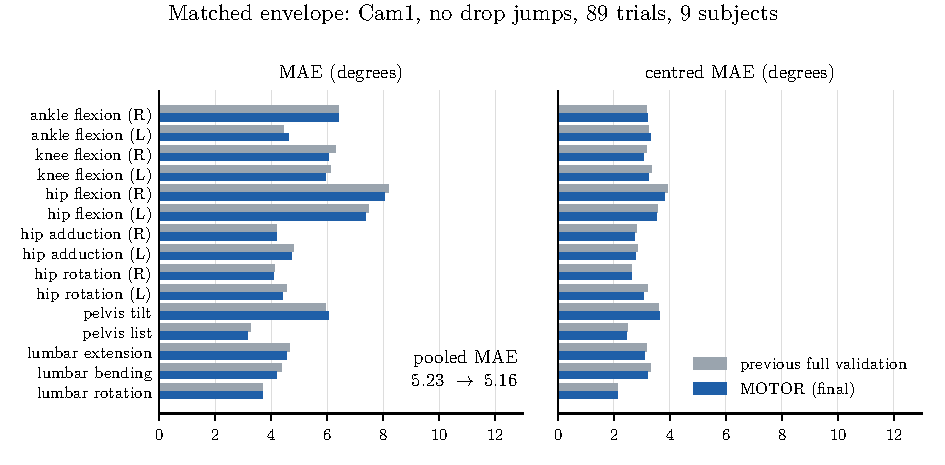
\includegraphics[width=\linewidth]{figures/angles-bars.pdf}
\caption{MOTOR's per-coordinate MAE and centred MAE on the matched set, beside MOTOR's previous full run of the same
inputs (before changes to its contact, floor and knee ligaments), scored with the same code.}
\label{fig:angles}
\end{figure}

\begin{figure}[h]
\centering
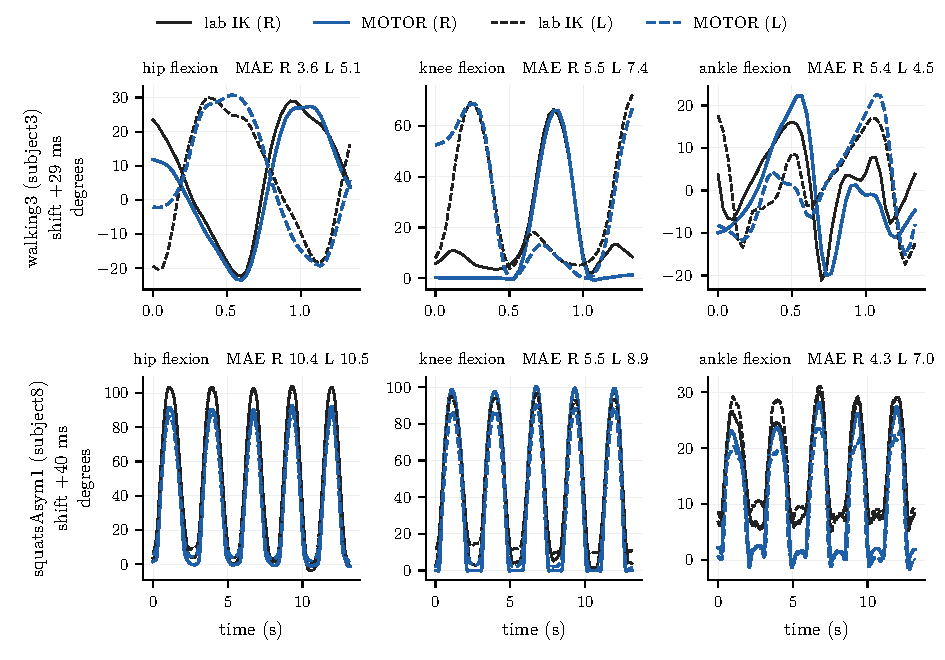
\includegraphics[width=\linewidth]{figures/waveforms.pdf}
\caption{MOTOR's hip, knee and ankle flexion in the 45\dg{} camera's median walking and squat trial (by angle error)
against the lab's inverse kinematics moved by the scored time shift.}
\label{fig:waveforms}
\end{figure}
% Figures restored from commit 096ac587 (paper/motor/figures/angles-bars.pdf, waveforms.pdf; made in commit 244bae78
% from the run of paper/motor/evidence/labval-final-2026-11-07.txt and its previous full run).

\FloatBarrier
\subsection{Per subject group, activity and camera}
\begin{center}\small
\captionof{table}{Per group: inputs, matched MAE and cMAE (degrees), vertical GRF MAE (\% body weight, both feet),
median vertical $r$ per foot over the trials where it is defined, joint moment MAE over OpenCap's 15 (\% weight
$\times$ height), mean EMG $r$ over the 16 channels. Cameras: LabValidation's numbering; Cam1 is the envelope's 45\dg{}
camera.}
\begin{tabular}{@{}lccccccc@{}}
\toprule
Group & $n$ & MAE & cMAE & GRF vert. & $r$ R / L & Moments & EMG $r$ \\
\midrule
held out 7--11 & 397 & 5.13 & 3.02 & 16.24 & 0.77 / 0.79 & 2.35 & 0.24 \\
training 2--5 & 319 & 5.63 & 3.54 & 16.09 & 0.78 / 0.77 & 2.37 & 0.22 \\
walking & 135 & 4.38 & 2.92 & 19.56 & 0.81 / 0.79 & 1.83 & 0.27 \\
walking (trunk sway) & 135 & 4.67 & 3.05 & 16.29 & 0.82 / 0.84 & 1.68 & 0.27 \\
squats & 87 & 5.79 & 3.26 & 6.25 & 0.52 / 0.47 & 1.55 & 0.17 \\
sit-to-stand & 90 & 5.39 & 2.92 & 11.28 & 0.69 / 0.81 & 1.51 & 0.20 \\
drop jump & 269 & 6.03 & 3.62 & 19.27 & 0.78 / 0.78 & 3.51 & 0.22 \\
Cam0 & 144 & 5.21 & 3.14 & 14.88 & 0.74 / 0.83 & 2.38 & 0.22 \\
Cam1 (45\dg) & 143 & 5.63 & 3.34 & 15.49 & 0.73 / 0.81 & 2.49 & 0.22 \\
Cam2 & 143 & 5.35 & 3.53 & 15.48 & 0.81 / 0.82 & 2.15 & 0.25 \\
Cam3 & 143 & 5.35 & 3.20 & 15.91 & 0.80 / 0.70 & 2.39 & 0.23 \\
Cam4 & 143 & 5.23 & 3.05 & 19.14 & 0.78 / 0.74 & 2.38 & 0.22 \\
\bottomrule
\end{tabular}
\end{center}
% moments-labval-2026-11-09.txt, the "after (all its trials)" column of each group's section ("held out 7-11, all",
% "training 2-5, all", "activity ...", "camera ..."): matched angle MAE and cMAE, GRF both vertical MAE, forces
% right/left vertical r (median over defined), joint moments, EMG r mean.

\subsection{Ground reaction force}
\begin{figure}[h]
\centering
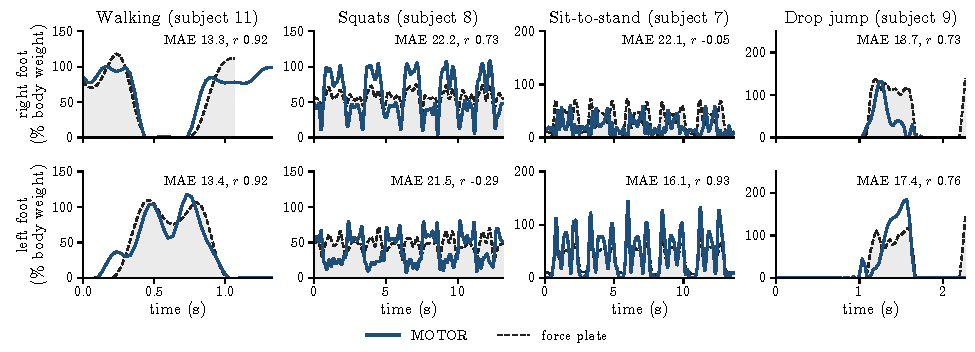
\includegraphics[width=\linewidth]{figures/grf-activities.pdf}
\caption{Vertical ground force under the right (top) and left foot (bottom), MOTOR (solid) against the plates
(dashed), in the median recording of each activity from the 45\dg{} camera (held-out subjects), with per-foot MAE
(\% body weight) and $r$.}
\label{fig:grf}
\end{figure}
% Trials subject11_walking4_Cam1, subject8_squats1_Cam1, subject7_STS1_Cam1, subject9_DJ1_Cam1: each the median of the
% 45 deg camera's trials of its activity (27, 17, 18, 52) by both-feet vertical MAE in the 2026-11-07 run's report.json;
% the panels' MAE and r reproduce report.json (e.g. subject9_DJ1_Cam1 right 18.677 / 0.734, left 17.386 / 0.759).
\begin{center}\small
\captionof{table}{Ground reaction force per activity, all five cameras: MAE in \% body weight on three axes with
both feet summed, filtered as OpenCap filters it, the activities' means weighted equally as OpenCap's, and the share of the plate's stance frames on which MOTOR's foot carries force.}
\begin{tabular}{@{}lccccc@{}}
\toprule
Activity & vertical & anterior & medio-lateral & 3-axis mean & stance carried R / L \\
\midrule
all & 16.18 & 7.43 & 2.99 & 8.9 & 0.82 / 0.79 \\
walking & 19.56 & 12.03 & 3.00 & 11.5 & 0.82 / 0.75 \\
walking (trunk sway) & 16.29 & 10.86 & 3.41 & 10.2 & 0.83 / 0.85 \\
squats & 6.25 & 3.53 & 3.31 & 4.4 & 0.99 / 0.95 \\
sit-to-stand & 11.28 & 4.51 & 3.27 & 6.4 & 0.82 / 0.82 \\
drop jump & 19.27 & 5.64 & 2.56 & 9.2 & 0.76 / 0.71 \\
\midrule
mean of the four activities & 13.68 & 6.28 & 3.09 & 7.7 & -- \\
\quad without drop jumps & 11.82 & 6.49 & 3.26 & 7.2 & -- \\
OpenCap, 2 cameras, mean & 11.4 & 3.5 & 3.8 & 6.2 & -- \\
\quad without drop jumps & 6.8 & 1.8 & 3.3 & 4.0 & -- \\
\bottomrule
\end{tabular}
\end{center}
% moments-labval-2026-11-09.txt, after columns ("all", "activity ...": GRF both vertical, anterior-posterior,
% medial-lateral, 3-axis mean, stance carried); the means of the activities: comparison-2026-11-09.txt ("all five",
% mean, 4 activities and no drop jumps; OpenCap's from its last section; 3-axis: the mean of the three).
Per foot over all 716 inputs, the vertical force's MAE is 17.8\% of body weight on the right and 17.2\% on the left.
In the 7 November run, the centre of pressure, with each trial's constant offset removed, was 47.6\,mm off in the
anterior and 20.2\,mm in the medio-lateral direction, and each stance's vertical impulse 12.6\% below the plate's on
average.
% Per foot: moments-labval-2026-11-09.txt ("all", after: GRF right vertical MAE 17.84, left 17.24). Centre of pressure
% and impulse: paper/motor/evidence/motor-labval-2026-11-09.txt ("GRF and centre of pressure, all trials, chain": the
% same 715 runs of 2026-11-07 scored by the same code; cop anterior-posterior centred mae
% 47.563 mm, medial-lateral 20.237 mm, impulse vertical error % of plate -12.594).

\subsection{Joint moments}
\begin{table}[h]
\centering\small
\caption{Joint moment MAE (\% weight $\times$ height) and $r$ per coordinate over all 715 inputs of the 7 November
run, before the two fixes, against OpenSim's inverse dynamics on the lab's own model. OpenCap's published mean over
its 15: 1.2.}
\begin{tabular}{@{}lcc@{\hspace{2em}}lcc@{}}
\toprule
Coordinate & MAE & $r$ & Coordinate & MAE & $r$ \\
\midrule
hip flexion r & 4.06 & 0.53 & hip flexion l & 3.82 & 0.53 \\
hip adduction r & 1.97 & 0.21 & hip adduction l & 1.86 & 0.16 \\
hip rotation r & 0.80 & 0.11 & hip rotation l & 0.76 & 0.13 \\
knee angle r & 2.83 & 0.39 & knee angle l & 2.71 & 0.37 \\
ankle angle r & 2.00 & 0.48 & ankle angle l & 2.01 & 0.36 \\
subtalar angle r & 0.65 & 0.43 & subtalar angle l & 0.57 & 0.40 \\
lumbar extension & 5.39 & 0.38 & elbow flex r & 0.19 & 0.40 \\
lumbar bending & 3.62 & 0.27 & elbow flex l & 0.23 & 0.43 \\
lumbar rotation & 3.14 & 0.27 & pro sup r / l & 0.02 / 0.02 & 0.10 / 0.10 \\
\midrule
OpenCap's 15, mean & 2.41 & & & & \\
\bottomrule
\end{tabular}
\end{table}
% paper/motor/evidence/motor-labval-2026-11-09.txt ("joint moments, all trials, chain": the same 715 runs of 2026-11-07
% scored by the same code, "coordinates <name> mae %bw.ht" mean and "r"); the mean of OpenCap's 15:
% labval-final-2026-11-07.txt ("all", 2.41); OpenCap's 1.2: the same file ("OpenCap's published figures").
After the two fixes the back's moments fall from 5.39, 3.62 and 3.14 to 4.83, 3.29 and 3.07\% of weight times height
(extension, bending, rotation), and the mean over OpenCap's 15 from 2.41 to 2.36\%; the fix to the torso's centre of
mass alone leaves it at 2.43\%, so the gain is the back's moment read at L5/S1.
% moments-labval-2026-11-09.txt, section 3 ("Effects separated": before 2.41, the RRA fix alone 2.43, with the back's
% own moment 2.36; lumbar extension, bending, rotation before 5.39, 3.62, 3.14, after 4.83, 3.29, 3.07).
In walking, the early-stance knee adduction moment's peak is overestimated: on the left knee MOTOR's mean is 3.4\%
of weight times height against the lab's 2.1\%, a mean error of 1.5\%. From the 45\dg{} camera, both knees together,
the first peak's error is 1.97\%, against OpenCap Monocular's 0.36\% and two-camera OpenCap's 0.41\% (0.30\% in
OpenCap's own paper); from Cam3 it is 0.75\%. In the
recorded runs, the knee of the leg far from the camera sits 37 to 44\,mm from the centre of pressure in the frontal
plane where the lab has 9 to 16\,mm, which accounts for most of this error.
% moments-labval-2026-11-09.txt ("all", after: early-stance kam l: mae 1.505, mean run 3.435, mean reference 2.051);
% Per camera: comparison-2026-11-09.txt ("walking's early-stance knee adduction moment peak": Cam1 1.97, Cam3 0.75;
% Monocular's 0.36 and 0.41 in its last section); OpenCap's 0.30: labval-final-2026-11-07.txt ("OpenCap's published
% figures"); far leg: #98 comment 6721835197.

\subsection{Where the moment error comes from}
\label{app:moments}
To separate the solver from its inputs, MOTOR's moment computation (the generalised forces each frame needs from
MuJoCo's inverse dynamics on the run's own model, less the ground force through the contact Jacobian, mapped onto the
coordinates) was run outside the pipeline on 159 trials (subjects 2, 4, 7, 9 and 11, every activity, the 45\dg{} camera
and Cam3, the runs before the fixes) with its two inputs, kinematics and ground force, each taken either from the
monocular run or from the laboratory: the lab's inverse kinematics low-passed at its inverse dynamics cutoff and
mapped onto MyoFullBody, and the plates' force and free moment with the centre of pressure carried from the lab's
ankle onto MyoFullBody's. Table~\ref{tab:moments-inputs} gives the result, scored as in the rest of this appendix.
\begin{table}[h]
\centering\small
\caption{Joint moment MAE over OpenCap's 15 (\% weight $\times$ height) from MOTOR's moment computation with each
input from the laboratory or from the monocular run; 159 trials. OpenCap's published errors: 2.50, 0.68, 0.97 and
0.75 in drop jumps, sit-to-stand, squats and walking, 1.22 over the four.}
\label{tab:moments-inputs}
\begin{tabular}{@{}llcccccc@{}}
\toprule
Kinematics & Ground force & all & drop jump & sit-to-stand & squats & walking & walking (sway) \\
\midrule
laboratory & laboratory & 1.28 & 2.41 & 0.47 & 0.42 & 0.66 & 0.80 \\
monocular & laboratory & 1.74 & 2.77 & 0.92 & 0.93 & 1.22 & 1.31 \\
laboratory & monocular & 2.24 & 3.65 & 1.28 & 1.35 & 1.49 & 1.49 \\
monocular & monocular & 2.41 & 3.65 & 1.57 & 1.58 & 1.78 & 1.71 \\
\bottomrule
\end{tabular}
\end{table}
% moments-labval-2026-11-09.txt, section 1 (rows 1, 2a, 2b, 0b; 0b reproduces the recorded run's 2.53 within 0.1-0.2);
% OpenCap's per activity: comparison-2026-11-09.txt, last section.
With the laboratory's inputs the computation is within 0.42 to 0.80\% of the laboratory's inverse dynamics outside
the drop jumps, whose remaining 2.41\% is the lumbar: the reference swings about 60\% of weight times height at
landing. Each monocular input alone leaves about half of the full error. The legs' moments carry the ground force's
error (hip flexion 3.7\% with the monocular force, 2.3\% with the monocular kinematics), the lumbar's only the
kinematics' (5.6\% with the monocular kinematics whatever the force, 3.9\% with the laboratory's). Reading the
back's moment at L5/S1 brought the laboratory-input figure from 1.28 to 1.19\%, the fix carried into the run.
% moments-labval-2026-11-09.txt, section 1 ("Answer", "Per coordinate", 1d: 1.28 to 1.19).

The ground force solve was checked the same way. Given the laboratory's kinematics, its first stage, the pelvis'
balance shared over a grid of sole points under each foot the plates show loaded, gives both feet's summed anterior
and medio-lateral forces within 2.33 and 2.25\% of body weight in walking (the plates' mean anterior magnitude is 8.1\%), and
1.06 and 0.57\% in squats, leaving a pelvis residual of 1.1\% of body weight; nothing in the solve suppresses the
horizontal force. The kinematics themselves decide it: the anterior force that the monocular kinematics demand
($m\mathbf{a} - m\mathbf{g}$ on the pelvis) is 17.4\% of body weight off the plates in walking, against 2.6\% with
the laboratory's. The split between two feet on the ground is not determined: each foot's anterior force in walking
is 5.5 to 6.0\% of body weight off with the laboratory's kinematics while their sum is right, since forces that
cancel between the feet do not act on the pelvis.
% moments-labval-2026-11-09.txt, section 2 (walking x 2.33, z 2.25, plates' mean |x| 8.1; squats 1.06 / 0.57;
% residual 1.1 %BW; demand x 17.4 against 2.6; per foot x 5.5-6.0 on walking).

\subsection{Residuals}
\begin{center}\small
\captionof{table}{The pelvis residual per group: the median over trials of each trial's median force (\% body weight)
and moment (\% weight $\times$ centre-of-mass height), the median of each trial's 95th-percentile force, and the mean
share of frames within both limits (2\% body weight, 1\% weight $\times$ centre of mass height). No trial is within
them on every frame.}
\begin{tabular}{@{}lccccc@{}}
\toprule
Group & trials & force & moment & force, 95th pct. & frames within \\
\midrule
all & 716 & 7.2 & 8.92 & 24.2 & 0.204 \\
held out 7--11 & 397 & 7.3 & 9.43 & 24.2 & 0.211 \\
walking & 135 & 8.1 & 11.00 & 23.1 & 0.062 \\
walking (trunk sway) & 135 & 7.2 & 9.89 & 20.2 & 0.071 \\
squats & 87 & 0.9 & 1.21 & 8.4 & 0.485 \\
sit-to-stand & 90 & 0.3 & 2.87 & 9.1 & 0.460 \\
drop jump & 269 & 11.0 & 9.38 & 85.6 & 0.166 \\
\bottomrule
\end{tabular}
\end{center}
% moments-labval-2026-11-09.txt ("residuals (after)"; frames within: each group's "residual: frames within limits",
% after; "share of trials within limits" 0.00).

\subsection{Muscle activations against EMG}
\begin{center}\small
\captionof{table}{Each EMG channel against MOTOR's activation of that muscle, all 715 inputs of the 7 November run
(over the 716 after the fixes the mean $r$ is unchanged at 0.23, its range $-0.07$ to 0.42): the share of frames on
which both are on or both off, Pearson's $r$, and the lag (s) at the cross-correlation peak.}
\begin{tabular}{@{}lccc@{\hspace{2em}}lccc@{}}
\toprule
Muscle & on/off & $r$ & lag & Muscle & on/off & $r$ & lag \\
\midrule
bflh l & 0.65 & 0.13 & -0.130 & semiten r & 0.70 & 0.23 & -0.034 \\
bflh r & 0.65 & 0.13 & -0.144 & soleus l & 0.70 & 0.26 & -0.030 \\
gasmed l & 0.70 & 0.23 & -0.009 & soleus r & 0.69 & 0.28 & -0.041 \\
gasmed r & 0.69 & 0.26 & -0.022 & tibant l & 0.59 & 0.22 & +0.031 \\
glmed1 l & 0.51 & 0.13 & +0.051 & vaslat l & 0.72 & 0.40 & -0.003 \\
glmed1 r & 0.52 & 0.15 & +0.040 & vaslat r & 0.72 & 0.42 & -0.018 \\
recfem l & 0.56 & -0.08 & -0.002 & vasmed l & 0.72 & 0.36 & -0.024 \\
semiten l & 0.66 & 0.18 & -0.053 & vasmed r & 0.76 & 0.41 & -0.033 \\
\bottomrule
\end{tabular}
\end{center}
% labval-final-2026-11-07.txt ("EMG per channel, all 715 trials (after)"); after the fixes: moments-labval-2026-11-09.txt
% ("all", after: EMG r, mean over channels 0.23 (-0.07 to 0.42)).

\begin{center}\small
\captionof{table}{OpenCap's vasti symmetry index in squats, per camera, in the 7 November run: the AUC of MOTOR's index against the asymmetry
the instructions asked for and against the EMG's own label (index over 1.15). OpenCap: 0.83 against the EMG label,
from its two cameras at $\pm$45\dg, the positions of Cam1 and Cam3.}
\begin{tabular}{@{}lcc@{}}
\toprule
Camera & AUC, instructed & AUC, EMG label \\
\midrule
Cam0 & 0.84 & 0.75 \\
Cam1 & 0.72 & 0.62 \\
Cam2 & 0.95 & 0.84 \\
Cam3 & 0.90 & 0.83 \\
Cam4 & 0.81 & 0.48 \\
all & 0.73 & 0.66 \\
\bottomrule
\end{tabular}
\end{center}
% labval-final-2026-11-07.txt ("vasti symmetry, after"); Cam1 and Cam3 the +-45 deg pair: comparison-2026-11-09.txt
% (its first section, from the dataset's calibration); OpenCap's pair: Uhlrich et al. 2023 via #98 comment 6744969345.

\subsection{Time per step}
\begin{center}\small
\captionof{table}{MOTOR's wall seconds per step on one NVIDIA L4, over the 715 runs of 7 November: median, range, and the median per
frame (clips of 30\,Hz).}
\begin{tabular}{@{}lcccc@{}}
\toprule
Step & median s & min s & max s & s per frame \\
\midrule
fit & 21.825 & 14.483 & 623.317 & 0.303 \\
set-up: physics model, GPU arrays, filtered path & 4.697 & 3.878 & 32.851 & 0.061 \\
footing & 4.669 & 1.758 & 35.312 & 0.062 \\
residual reduction, iterations & 19.862 & 5.910 & 392.306 & 0.246 \\
residual reduction, tracking and per-frame caps & 4.603 & 1.714 & 45.888 & 0.061 \\
checks: residual record, feet on the floor, tracking & 2.120 & 1.111 & 17.879 & 0.028 \\
static optimisation, stage 1 (ground reaction) & 3.003 & 0.114 & 28.318 & 0.034 \\
static optimisation, stage 2 (joint limits and muscles) & 2.296 & 1.169 & 22.356 & 0.032 \\
inverse dynamics, contacts and muscle paths & 1.120 & 0.356 & 12.459 & 0.013 \\
writing records and force measures & 0.264 & 0.042 & 2.639 & 0.003 \\
saving arrays & 0.005 & 0.003 & 0.012 & 0.000 \\
total & 66.214 & 34.843 & 788.668 & 0.871 \\
\bottomrule
\end{tabular}
\end{center}
% labval-final-2026-11-07.txt ("sim body wall seconds per step, after").

\begin{table}[h]
\centering\small
\caption{Wall time per trial, MOTOR against published solves. OpenCap's solves are those recorded in its
LabValidation release, timed by us (80 muscles, windows of 0.99 to 1.68\,s, solve only, hardware not recorded); its
paper reports 37\,min for one squat on one server. MOTOR's time excludes the video pose estimate.}
\label{tab:timing}
\begin{tabular}{@{}lll@{}}
\toprule
Method & Clip & Wall time \\
\midrule
OpenCap solve \cite{uhlrich2023opencap} & walk, drop jump, squat & 4196, 4096, 2635\,s \\
Moco, MocoTrack \cite{dembia2020moco} & gait & about 130\,min \\
OpenSim CMC \cite{rajagopal2016fullbody} & gait & about 10\,min \\
MOTOR, one L4 & LabValidation, 715 trials & 66\,s median (35--789\,s) \\
\bottomrule
\end{tabular}
\end{table}
% OpenCap's solves, Moco's and CMC's times: #98 comment 6696117098 ("Timing comparison": OpenCap's Setup.yaml and
% Stats.npy, Dembia 2020, Rajagopal 2016); 37 min: 2 min kinematics and 35 min kinetics for one squat, Uhlrich et al.
% 2023, Results, field study (#98 comment 6744969345); MOTOR's row: labval-final-2026-11-07.txt ("sim body wall seconds per
% step": total median 66.214, min 34.843, max 788.668).

\begin{figure}[h]
\centering
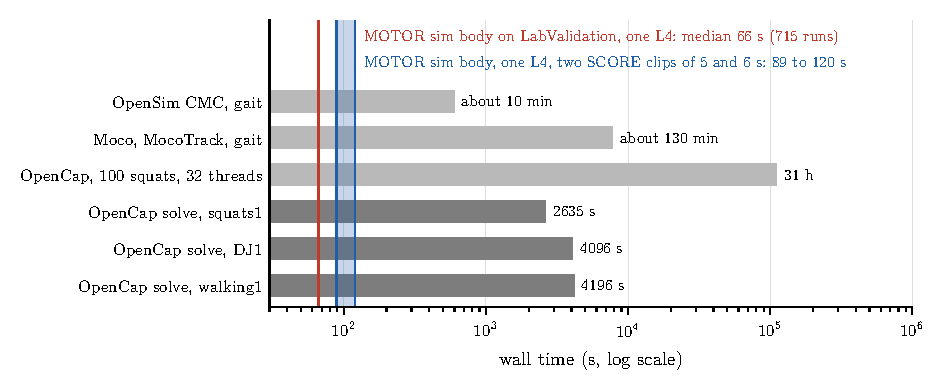
\includegraphics[width=\linewidth]{figures/timing.pdf}
\caption{MOTOR's wall time per trial on a log scale: OpenCap's recorded solves and published OpenSim times (grey),
MOTOR on two SCORE clips (blue band) and its median on LabValidation (red).}
\label{fig:timing}
\end{figure}
% Restored from commit 096ac587 (paper/motor/figures/timing.pdf, made in 244bae78): OpenCap's, Moco's and CMC's times
% from #98 comment 6696117098; MOTOR's band from paper/motor/evidence/speed-2026-11-06.txt; its median from
% labval-final-2026-11-07.txt.

\FloatBarrier
\subsection{What the run shows}

\paragraph{What the input carries.} MOTOR follows its input, so the input's errors pass through. The elbows come out
straighter than the lab's in every one of the 89 matched trials, by a mean 21.1\dg{} (right) and 23.7\dg{} (left),
with centred errors of 3.0 and 4.6\dg. On 540 walking arm trials GEM-X's own elbow is a median 18.5\dg{} straighter
than the markers', and the fit's elbow differs from GEM-X's by a median 2.5\dg. The pelvis tilt is offset in one
direction in 82 of 89 matched trials, by a mean 5.3\dg. Neither is calibrated away: no angle is fitted to the
reference, and reading each subject's own standing trial as a static calibration, tried on the held-out subjects, made
their pelvis tilt, elbows and matched error worse.
% paper/motor/evidence/elbow-2026-11-07.txt (540 walking arm-trials, SOMA minus markers median -18.5; sim body
% minus SOMA median -2.5); labval-final-2026-11-07.txt ("signed offsets": elbow r -21.12, l -23.66, 89 of 89; pelvis
% tilt +5.26, 82 of 89; per coordinate: envelope cMAE elbow r 3.00, l 4.61); standing trial tried and not used:
% tools/labval/CLAUDE.md ("The subject's standing pose, tried and not used") and
% paper/motor/evidence/static-neutral-2026-11-08.txt.

\paragraph{Forces, residuals and the two sides.} The pelvis residual stays above its limits, the anterior ground
reaction force error is about twice OpenCap's over its four activities and nearly four times without drop jumps, and the activation pattern is partly off (rectus femoris does not
follow its EMG, $r=-0.08$). The ground force is split between the feet by the skin points that reach the floor and by
the pelvis' balance, so a foot that GEM-X places a little higher carries less: in the squat of
Figure~\ref{fig:teaser}, at its deepest frame, the left foot carries 90\% of body weight and the right 53\%, and the
calf muscles follow that split rather than the symmetric movement.
% labval-final-2026-11-07.txt ("residuals", "all", "EMG per channel"); anterior against OpenCap:
% comparison-2026-11-09.txt ("Cam1+Cam3" 6.48 against 3.5, 6.75 against 1.8); teaser-2026-11-07.json (frame 216: left 90.13,
% right 52.93 %BW); inside/contact/__init__.py (STANCE_HIGH comment: GEM-X's standing sole 18 to 28 mm up).

\paragraph{Camera sampling and fast movements.} GEM-X resamples every clip to 30\,Hz, so an impact or a push-off is
sampled at that rate whatever the phone recorded. Of the five activities the drop jumps have the highest joint moment
error (3.51\% of weight times height, against 1.51 to 1.83 for the others) and the largest pelvis residual (a median of
11.0\% of body weight, its 95th percentile 85.6\%).
% 30 Hz: tools/labval/_soma.py RATE. Drop jumps: moments-labval-2026-11-09.txt (after: "activity ..." moments drop jump
% 3.51, walking 1.83, sit-to-stand 1.51; "residuals (after)" drop jump 11.0 and 85.6).

\paragraph{The fit's own records.} The calibration (level 1) tunes on synthetic SOMA bodies, not on people. The last
calibration run whose held-out score is recorded met its rule: its check bodies' score fell from 4.26 to 3.56 while the tuning bodies' fell
from 4.53 to 3.44, and the rule's comparison, 3.56 against the tuning bodies' 3.51, was within 10\%. The tuned point
the fit uses now came from a later run with a broader objective, whose held-out score is not yet recorded. The bones
are not yet all inside the skin: on the fifteen clips of the synthetic body of mean shape, 5.15\% of the bone points
lie outside it (averaged over body regions), against a target of under 5\%.
% Level 1 run l1e: #70 comment 6556935709 ("C. Level 1 runs": tuning 4.5259 to 3.4404, check 4.2602 to 3.5597,
% "within 10 %: yes (3.56 against 3.51)"); the point in use, run l1n: #70 comment 6621931172; 5.15 %: #70 comment
% 6629418159 (commit 0efb7213); target under 5 %: #70 comment 6565739270.

\FloatBarrier
\subsection{Failures}
\label{app:failures}

\begin{center}\small
\captionof{table}{The 4 of 720 inputs without a score, by cause.}
\begin{tabular}{@{}lr@{}}
\toprule
Cause & Inputs \\
\midrule
The GPU fit did not stop in 3000 iterations (subject 10, squats1, two cameras) & 2 \\
Passed its job's time limit (subject 10, squats1, a third camera; subject 5, a drop jump) & 2 \\
\midrule
Total & 4 \\
\bottomrule
\end{tabular}
\end{center}
% moments-labval-2026-11-09.txt, section 3 (716 of 720: subject10_squats1 Cam1 and Cam4, the fit did not stop in 3000
% steps; subject10_squats1_Cam3 and subject5_DJAsym3_Cam2, their job's time).
\clearpage
\section{Model and solver parameters}
\label{app:parameters}
\begin{center}\small
\captionof{table}{The bone groups: each SOMA segment, the MyoFullBody bone that carries its rotation, and the bones
the group covers. Every sided group exists on both sides; 7 middle and 7 sided groups make 21, of which 20 drive their
frame bone.}
\begin{tabular}{@{}lll@{}}
\toprule
SOMA segment & Frame bone & Bones in the group \\
\midrule
Hips & pelvis & pelvis, sacrum \\
Spine1 & lumbar 4 & lumbar 5 and 4 \\
Spine2 & lumbar 1 & lumbar 3 to 1 \\
Chest & torso & torso, thorax, cervical spine \\
Neck1 & neck & neck \\
Neck2 & neck (drives nothing) & -- \\
Head & head & head \\
Shoulder & scapula & clavicle, scapula \\
Arm & humerus & humerus \\
ForeArm & ulna & ulna, radius \\
Hand & lunate & carpals, metacarpals, phalanges \\
Leg & femur & femur \\
Shin & tibia & tibia \\
Foot & calcaneus & talus, calcaneus \\
ToeBase & toes & toes \\
\bottomrule
\end{tabular}
\end{center}
% score/stages/sim_body/inside/bone_groups/__init__.py (GROUPS; the shoulder's and arm's helper bodies of MoBL-ARMS
% are left out of the list); Neck2 drives none: inside/fit/CLAUDE.md ("One segment drives one bone group").

\begin{center}\small
\captionof{table}{MOTOR's parameters in one place.}
\begin{tabular}{@{}lll@{}}
\toprule
Part & Parameter & Value \\
\midrule
Model & muscles, bones, joints & 416, 86, 132 \\
 & joints: root, coupled, free & 1, 36, 95 \\
Landmarks & defined, used by the fit & 102, 84 \\
Fit & markers' goal $\lambda_m$ & 2.1169 \\
 & skin goal $\lambda_s$ & $10^3$ \\
 & most steps per frame & 300 \\
Level 1 & segment end's reach & 40\,mm \\
 & held-out rule & check bodies within 10\% of tuning bodies \\
Level 2 & sampled frames & about 30 \\
 & landmark's and inside joint's reach & 3\,cm \\
Forces & contact gap & 5\,mm \\
 & a seen standing foot pushed up to & 5\,cm over the floor \\
 & ground share weight, rounds & 0.03 per newton, 2 \\
 & smoothing cut-off & 6\,Hz \\
 & residual reduction: rounds & 3 \\
 & \quad per-frame cap & 5\dg{} per segment, 2\,cm at the pelvis \\
 & \quad mass change & at most 2\% \\
 & residual limits & 2\% body weight; 1\% weight $\times$ centre of mass height \\
\bottomrule
\end{tabular}
\end{center}
% Model: paper/motor/evidence/model-2026-11-06.txt; landmarks: inside/landmarks/CLAUDE.md; fit: inside/fit/_frames.py
% (MARKER_GOAL, MOST_STEPS), inside/fit/_skin.py (SKIN_GOAL); level 1: inside/tuning/CLAUDE.md (END_REACH), #70
% comment 6556935195; level 2: inside/fit/__init__.py SAMPLE, inside/fit/_constants.py MARK_MOST; forces:
% inside/contact/__init__.py (GAP, STANCE_HIGH), inside/muscles/__init__.py (SHARE_COST, SHARE_ROUNDS),
% inside/solvers/__init__.py CUTOFF, inside/rra/__init__.py (RRA_ROUNDS, MASS_MOST), _gates.py (FOLLOWED,
% MOVE_MOST); limits: score/stages/sim_body/CLAUDE.md.

\section{Disclosure, data and code}
\label{sec:availability}

The code of MOTOR and of its validation was written by a coding agent (Claude Code) under the author's direction and
review; this draft was written the same way. No reported measure was hand-picked: Figure~\ref{fig:teaser} shows
chosen recordings, Figure~\ref{fig:grf} medians. The only settings chosen on LabValidation
(MOTOR's contact gap, the height from which a seen standing foot is pushed, the weight that shares the ground force
over the touching points, and the clearance of a drop jump's box) were chosen on subjects 2 to 5 against their force
plates, never against joint angles; subjects 7 to 11 were never used to choose any setting. Of these, only the
standing foot's height changed from its first value, from 30 to 50\,mm.
% labval-final-2026-11-07.txt ("tuning": arms A to E on 36 Cam1 trials of subjects 2-5, C chosen, commit a40b66d6;
% the box's 0.10 m clearance, commit 11edb366; header: "Held out: subjects 7 to 11 were never used to choose any
% setting").

MOTOR and this paper's sources are open under the MIT licence at
\url{https://github.com/Babon-Innovations-b-v/motor}, and its validation tools at
\url{https://github.com/Babon-Innovations-b-v/score}; every number in this paper is read from a file or record named in
a comment beside it in the paper's source. We collected no new data from people. LabValidation is the public release
of OpenCap's authors \cite{uhlrich2023opencap}, used under its Apache-2.0 licence and fetched on demand, never
redistributed.
% LabValidation licence: #57 comment 6441121325 (Apache-2.0, fetched on demand, never committed); MIT: LICENSE.

\end{document}
